\documentclass[11pt,a4paper]{article}
% ==== begin preamble ====
% ============================================================================
% preamble.tex -- Self-reinforced geometric absorption
% Engine: pdflatex (see latexmkrc).  Bibliography: biblatex + biber, style=phys
% ============================================================================

% ---- Layout & typography ---------------------------------------------------
\usepackage[a4paper,margin=2.5cm,headheight=14pt]{geometry}
\usepackage[T1]{fontenc}
\usepackage[utf8]{inputenc}
\usepackage{lmodern}
\usepackage{microtype}
\usepackage{csquotes}

% ---- Mathematics -----------------------------------------------------------
\usepackage{amsmath}
\usepackage{amssymb}
\usepackage{amsthm}
\usepackage{mathtools}
\usepackage{bm}
\usepackage{mathrsfs}   % \mathscr, used for the Hilbert space
\usepackage{tensor}

% ---- Graphics & tables -----------------------------------------------------
\usepackage{graphicx}
\usepackage{float}
\usepackage[font=small,labelfont=bf,labelsep=period]{caption}
\usepackage{subcaption}
\graphicspath{{figures/}}
\usepackage{booktabs}
\usepackage{array}
\usepackage{longtable}
\usepackage{tabularx}
\usepackage{multirow}
\usepackage[group-separator={,},group-minimum-digits=4,detect-all]{siunitx}
\newcolumntype{L}[1]{>{\raggedright\arraybackslash}p{#1}}
\newcolumntype{C}[1]{>{\centering\arraybackslash}p{#1}}
\newcolumntype{Y}{>{\raggedright\arraybackslash}X}

% ---- Lists, spacing, floats ------------------------------------------------
\usepackage{enumitem}
\usepackage{xspace}
\usepackage{etoolbox}
\usepackage[section]{placeins}
\usepackage{needspace}
\usepackage{xcolor}

% ---- Links (load before cleveref) ------------------------------------------
\usepackage[colorlinks=true,linkcolor=blue!55!black,citecolor=green!45!black,
            urlcolor=black!65,bookmarks=true,bookmarksnumbered=true]{hyperref}
\usepackage[nameinlink,capitalise]{cleveref}

% ---- Bibliography ----------------------------------------------------------
\usepackage[backend=biber,style=phys,biblabel=brackets,sorting=none,
            eprint=true,doi=true,url=false,isbn=false,
            maxbibnames=5,minbibnames=3,giveninits=true]{biblatex}
% bibliography is shipped as main.bbl

% ============================================================================
% Draft-figure guard.  In draft mode a missing figure prints a visible box;
% in final mode a missing figure is a hard error (never silently dropped).
% ============================================================================
\newif\ifdraftfigs
\draftfigstrue   % <-- set \draftfigsfalse before submission
\let\origincludegraphics\includegraphics
\renewcommand{\includegraphics}[2][]{%
  \IfFileExists{figures/#2}%
    {\origincludegraphics[#1]{#2}}%
    {\ifdraftfigs
       \fbox{\parbox{0.6\linewidth}{\centering\color{red}\ttfamily
             MISSING FIGURE\\ figures/#2}}%
     \else
       \GenericError{}{Missing figure: figures/#2}{}{Build aborted: final mode requires all figures.}%
     \fi}}

% ============================================================================
% Theorem environments (shared counter, numbered by section)
% ============================================================================
\theoremstyle{plain}
\newtheorem{theorem}{Theorem}[section]
\newtheorem{proposition}[theorem]{Proposition}
\newtheorem{lemma}[theorem]{Lemma}
\newtheorem{corollary}[theorem]{Corollary}
\theoremstyle{definition}
\newtheorem{definition}[theorem]{Definition}
\newtheorem{assumption}[theorem]{Assumption}
\newtheorem{example}[theorem]{Example}
\newtheorem{conjecture}[theorem]{Conjecture}
\theoremstyle{remark}
\newtheorem{remark}[theorem]{Remark}
\newtheorem{notation}[theorem]{Notation}

\crefname{theorem}{Theorem}{Theorems}
\crefname{proposition}{Proposition}{Propositions}
\crefname{lemma}{Lemma}{Lemmas}
\crefname{corollary}{Corollary}{Corollaries}
\crefname{definition}{Definition}{Definitions}
\crefname{assumption}{Assumption}{Assumptions}
\crefname{conjecture}{Conjecture}{Conjectures}
\crefname{remark}{Remark}{Remarks}
\crefname{equation}{Eq.}{Eqs.}
\crefname{figure}{Fig.}{Figs.}
\crefname{table}{Table}{Tables}
\crefname{section}{Sec.}{Secs.}
\crefname{appendix}{Appendix}{Appendices}

\numberwithin{equation}{section}

% ============================================================================
% Claims ladder.  Every displayed key result is wrapped in `keyresult`, whose
% level is machine-extracted by scripts/check_claims.py:
%   I = identity or standard result   C = conditional theorem of the model
%   P = phenomenological / fitted     S = speculative (Outlook only)
% Usage:  \begin{keyresult}{C}{eq:jerk-bound} ... \end{keyresult}
% ============================================================================
\newenvironment{keyresult}[2]%
  {\begin{equation}\label{#2}\begin{aligned}}%
  {\end{aligned}\end{equation}}
% The level argument #1 is not typeset; it is extracted from the source by
% scripts/check_claims.py, which greps \begin{keyresult}{LEVEL}{label}.

% ---- Draft helpers (removed before submission) ------------------------------
\newcommand{\TODO}[1]{\textcolor{red}{\textbf{[TODO: #1]}}}
\newcommand{\CITE}{\textcolor{orange}{\textbf{[CITE]}}}

% ==== end preamble ====
% ==== begin macros ====
% ============================================================================
% macros.tex -- notation for self-reinforced geometric absorption
% Notation clashes resolved here (see docs/NOTATION.md):
%   \Gam   = conversion rate        (Christoffel written explicitly)
%   \Mmem  = memory variable        (\Mpl = reduced Planck mass)
%   \bfrac = branching ratio        (baryons carry subscript \mathrm{b})
%   \clock = constrained clock T    (stress tensor is \Tmn)
% ============================================================================

% ---- Calculus --------------------------------------------------------------
\newcommand{\dd}{\mathrm{d}}
\newcommand{\pdv}[2]{\frac{\partial #1}{\partial #2}}
\newcommand{\odv}[2]{\frac{\dd #1}{\dd #2}}
\newcommand{\pdvat}[2]{\partial_{#2} #1}
\DeclareMathOperator{\Ei}{Ei}
\DeclareMathOperator{\csch}{csch}
\DeclareMathOperator{\sech}{sech}
\DeclareMathOperator{\Tr}{Tr}
\DeclareMathOperator{\sgn}{sgn}
\DeclareMathOperator*{\argmin}{arg\,min}
\newcommand{\order}[1]{\mathcal{O}\!\left(#1\right)}
\newcommand{\eqdef}{\coloneqq}
\newcommand{\abs}[1]{\left|#1\right|}
\newcommand{\norm}[1]{\left\lVert#1\right\rVert}
\newcommand{\avg}[1]{\left\langle #1 \right\rangle}

% ---- Gravity / geometry ----------------------------------------------------
\newcommand{\Mpl}{M_{\mathrm{Pl}}}
\newcommand{\Lag}{\mathcal{L}}
\newcommand{\Sact}{S}
\newcommand{\gdet}{\sqrt{-g}}
\newcommand{\covd}{\nabla}
\newcommand{\Tmn}{T_{\mu\nu}}
\newcommand{\Tup}{T^{\mu\nu}}
\newcommand{\Tof}[1]{T^{(#1)}_{\mu\nu}}
\newcommand{\Gmn}{G_{\mu\nu}}
\newcommand{\umu}{u^{\mu}}
\newcommand{\ulow}{u_{\mu}}
\newcommand{\proj}{\Delta^{\mu\nu}}
\newcommand{\expa}{\Theta}
\newcommand{\clock}{T}                       % constrained clock field
\newcommand{\lagm}{\lambda}                  % Lagrange multiplier
\newcommand{\fourform}{\mathcal{H}}          % four-form field strength

% ---- Cosmological densities ------------------------------------------------
\newcommand{\rhoI}{\rho_{I}}                 % precursor
\newcommand{\rhoD}{\rho_{D}}                 % localized defects
\newcommand{\rhoV}{V}                        % vacuum energy density
\newcommand{\rhob}{\rho_{\mathrm{b}}}        % baryons
\newcommand{\rhor}{\rho_{\mathrm{r}}}        % radiation
\newcommand{\rhom}{\rho_{\mathrm{m}}}        % total dust
\newcommand{\rhotot}{\rho_{\mathrm{tot}}}
\newcommand{\rhodmeff}{\rho_{\mathrm{dm}}^{\mathrm{eff}}}
\newcommand{\Vinf}{V_{\infty}}
\newcommand{\Vearly}{V_{\mathrm{early}}}

% ---- Absorption kinetics ---------------------------------------------------
\newcommand{\Gam}{\Gamma}                    % conversion rate
\newcommand{\Gamz}{\Gamma_{0}}
\newcommand{\Gamdn}{\Gamma_{\downarrow}}     % reverse (Track B) channel
\newcommand{\fconv}{f}                       % converted fraction
\newcommand{\Mmem}{M}                        % memory variable
\newcommand{\tauM}{\tau_{M}}
\newcommand{\bfrac}{b}                       % branching ratio to defects
\newcommand{\QV}{Q_{V}}                      % energy transfer density-rate
\newcommand{\Qnet}{Q_{\mathrm{net}}}
\newcommand{\xieff}{\xi_{\mathrm{eff}}}
\newcommand{\actS}{S_{\mathrm{act}}}         % activation switch
\newcommand{\zact}{z_{\mathrm{act}}}
\newcommand{\aact}{a_{\mathrm{act}}}

% ---- Expansion & cosmography -----------------------------------------------
\newcommand{\Hub}{H}
\newcommand{\Hz}{H_{0}}
\newcommand{\Hinf}{H_{\infty}}
\newcommand{\Om}[1]{\Omega_{#1}}
\newcommand{\Omm}{\Omega_{\mathrm{m}}}
\newcommand{\Omr}{\Omega_{\mathrm{r}}}
\newcommand{\OmV}{\Omega_{V}}
\newcommand{\decel}{q}
\newcommand{\jerk}{j}
\newcommand{\snap}{s}
\newcommand{\efold}{N}
\newcommand{\weff}{w_{\mathrm{eff}}}
\newcommand{\dS}{de~Sitter\xspace}
\newcommand{\LCDM}{\Lambda\mathrm{CDM}}
\newcommand{\wCDM}{w\mathrm{CDM}}
\newcommand{\wzwa}{w_{0}w_{a}\mathrm{CDM}}

% ---- Distances & data ------------------------------------------------------
\newcommand{\DM}{D_{M}}
\newcommand{\DHub}{D_{H}}
\newcommand{\DV}{D_{V}}
\newcommand{\DL}{D_{L}}
\newcommand{\DA}{D_{A}}
\newcommand{\rdrag}{r_{\mathrm{d}}}
\newcommand{\rs}{r_{s}}
\newcommand{\zstar}{z_{*}}
\newcommand{\shift}{\mathcal{R}}             % CMB shift parameter
\newcommand{\lA}{\ell_{A}}
\newcommand{\fsig}{f\sigma_{8}}
\newcommand{\chisq}{\chi^{2}}
\newcommand{\lnL}{\ln\mathcal{L}}
\newcommand{\AIC}{\mathrm{AIC}}
\newcommand{\BIC}{\mathrm{BIC}}
\newcommand{\lnZ}{\ln\mathcal{Z}}
\newcommand{\lnB}{\ln B}

% ---- Probability & quantum -------------------------------------------------
\newcommand{\E}{\mathbb{E}}
\newcommand{\Prob}{\mathbb{P}}
\newcommand{\Var}{\mathrm{Var}}
\newcommand{\Real}{\mathbb{R}}
\newcommand{\Nat}{\mathbb{N}}
\newcommand{\Int}{\mathbb{Z}}
\newcommand{\Lind}{\mathcal{L}}              % Lindblad generator
\newcommand{\dens}{\varrho}                  % density matrix
\newcommand{\jump}{L}                        % jump operator
\newcommand{\Hilb}{\mathscr{H}}
% Dirac notation.  Defined here rather than loading physics.sty, which would
% redefine \dd, \abs, \norm and \vec and clash with the definitions above.
\newcommand{\ket}[1]{\lvert #1 \rangle}
\newcommand{\bra}[1]{\langle #1 \rvert}
\newcommand{\braket}[2]{\langle #1 \vert #2 \rangle}
\newcommand{\ketbra}[2]{\lvert #1 \rangle\!\langle #2 \rvert}

% ---- Defects ---------------------------------------------------------------
\newcommand{\Fstar}{F_{*}}
\newcommand{\kaps}{\kappa_{s}}
\newcommand{\Rs}{R_{s}}
\newcommand{\degB}{B}                        % topological degree

% ==== end macros ====
% ==== begin generated/numbers ====
% Auto-generated by scripts/gen_numbers.py from results/results.json.
% Do not edit by hand: `make tables` regenerates it and `make check`
% fails if the committed file disagrees with the results.
\newcommand{\numChainsLcdmBaselineAcceptance}{0.4574\xspace}
\newcommand{\numChainsLcdmBaselineAic}{1443\xspace}
\newcommand{\numChainsLcdmBaselineBic}{1459\xspace}
\newcommand{\numChainsLcdmBaselineBurnIn}{37\xspace}
\newcommand{\numChainsLcdmBaselineChiTBreakdownBAODESIDRT}{12.19\xspace}
\newcommand{\numChainsLcdmBaselineChiTBreakdownCCDefault}{6.27\xspace}
\newcommand{\numChainsLcdmBaselineChiTBreakdownCMBCompressed}{2.947\xspace}
\newcommand{\numChainsLcdmBaselineChiTBreakdownSNPantheon}{1415\xspace}
\newcommand{\numChainsLcdmBaselineChiTMin}{1437\xspace}
\newcommand{\numChainsLcdmBaselineConverged}{\text{true}\xspace}
\newcommand{\numChainsLcdmBaselineDataset}{baseline\xspace}
\newcommand{\numChainsLcdmBaselineDerivedFZ}{0\xspace}
\newcommand{\numChainsLcdmBaselineDerivedFZErrHi}{0\xspace}
\newcommand{\numChainsLcdmBaselineDerivedFZErrLo}{0\xspace}
\newcommand{\numChainsLcdmBaselineDerivedH}{0.6838\xspace}
\newcommand{\numChainsLcdmBaselineDerivedHErrHi}{0.002817\xspace}
\newcommand{\numChainsLcdmBaselineDerivedHErrLo}{0.002993\xspace}
\newcommand{\numChainsLcdmBaselineDerivedHZ}{68.38\xspace}
\newcommand{\numChainsLcdmBaselineDerivedHZErrHi}{0.2817\xspace}
\newcommand{\numChainsLcdmBaselineDerivedHZErrLo}{0.2993\xspace}
\newcommand{\numChainsLcdmBaselineDerivedJZ}{1\xspace}
\newcommand{\numChainsLcdmBaselineDerivedJZErrHi}{1.366e-06\xspace}
\newcommand{\numChainsLcdmBaselineDerivedJZErrLo}{1.27e-06\xspace}
\newcommand{\numChainsLcdmBaselineDerivedMZ}{0\xspace}
\newcommand{\numChainsLcdmBaselineDerivedMZErrHi}{0\xspace}
\newcommand{\numChainsLcdmBaselineDerivedMZErrLo}{0\xspace}
\newcommand{\numChainsLcdmBaselineDerivedMatterDeficit}{-0.001408\xspace}
\newcommand{\numChainsLcdmBaselineDerivedMatterDeficitErrHi}{1.153e-05\xspace}
\newcommand{\numChainsLcdmBaselineDerivedMatterDeficitErrLo}{1.241e-05\xspace}
\newcommand{\numChainsLcdmBaselineDerivedOmegaMEarly}{0.1402\xspace}
\newcommand{\numChainsLcdmBaselineDerivedOmegaMEarlyErrHi}{0.0006442\xspace}
\newcommand{\numChainsLcdmBaselineDerivedOmegaMEarlyErrLo}{0.0005888\xspace}
\newcommand{\numChainsLcdmBaselineDerivedOmegaMZ}{0.1409\xspace}
\newcommand{\numChainsLcdmBaselineDerivedOmegaMZErrHi}{0.0006442\xspace}
\newcommand{\numChainsLcdmBaselineDerivedOmegaMZErrLo}{0.0005888\xspace}
\newcommand{\numChainsLcdmBaselineDerivedOmegaRZ}{5.288e-05\xspace}
\newcommand{\numChainsLcdmBaselineDerivedOmegaRZErrHi}{4.659e-07\xspace}
\newcommand{\numChainsLcdmBaselineDerivedOmegaRZErrLo}{4.329e-07\xspace}
\newcommand{\numChainsLcdmBaselineDerivedOmegaVZ}{0.6987\xspace}
\newcommand{\numChainsLcdmBaselineDerivedOmegaVZErrHi}{0.003558\xspace}
\newcommand{\numChainsLcdmBaselineDerivedOmegaVZErrLo}{0.003882\xspace}
\newcommand{\numChainsLcdmBaselineDerivedQZ}{-0.548\xspace}
\newcommand{\numChainsLcdmBaselineDerivedQZErrHi}{0.005824\xspace}
\newcommand{\numChainsLcdmBaselineDerivedQZErrLo}{0.005337\xspace}
\newcommand{\numChainsLcdmBaselineDerivedVZMinusVact}{0\xspace}
\newcommand{\numChainsLcdmBaselineDerivedVZMinusVactErrHi}{0\xspace}
\newcommand{\numChainsLcdmBaselineDerivedVZMinusVactErrLo}{0\xspace}
\newcommand{\numChainsLcdmBaselineDerivedZAcc}{0.6726\xspace}
\newcommand{\numChainsLcdmBaselineDerivedZAccErrHi}{0.006157\xspace}
\newcommand{\numChainsLcdmBaselineDerivedZAccErrLo}{0.01225\xspace}
\newcommand{\numChainsLcdmBaselineModel}{lcdm\xspace}
\newcommand{\numChainsLcdmBaselineNData}{1{,}621\xspace}
\newcommand{\numChainsLcdmBaselineNParams}{3\xspace}
\newcommand{\numChainsLcdmBaselineNSteps}{2{,}000\xspace}
\newcommand{\numChainsLcdmBaselineNWalkers}{32\xspace}
\newcommand{\numChainsLcdmBaselineParametersOmegaBHiNV}{0.02276\xspace}
\newcommand{\numChainsLcdmBaselineParametersOmegaBHiXE}{0.02264\xspace}
\newcommand{\numChainsLcdmBaselineParametersOmegaBLoNV}{0.02228\xspace}
\newcommand{\numChainsLcdmBaselineParametersOmegaBLoXE}{0.0224\xspace}
\newcommand{\numChainsLcdmBaselineParametersOmegaBMean}{0.02252\xspace}
\newcommand{\numChainsLcdmBaselineParametersOmegaBMedian}{0.02252\xspace}
\newcommand{\numChainsLcdmBaselineParametersOmegaCHiNV}{0.119\xspace}
\newcommand{\numChainsLcdmBaselineParametersOmegaCHiXE}{0.1184\xspace}
\newcommand{\numChainsLcdmBaselineParametersOmegaCLoNV}{0.1164\xspace}
\newcommand{\numChainsLcdmBaselineParametersOmegaCLoXE}{0.1171\xspace}
\newcommand{\numChainsLcdmBaselineParametersOmegaCMean}{0.1177\xspace}
\newcommand{\numChainsLcdmBaselineParametersOmegaCMedian}{0.1177\xspace}
\newcommand{\numChainsLcdmBaselineParametersOmegaVActHiNV}{0.3355\xspace}
\newcommand{\numChainsLcdmBaselineParametersOmegaVActHiXE}{0.3312\xspace}
\newcommand{\numChainsLcdmBaselineParametersOmegaVActLoNV}{0.3178\xspace}
\newcommand{\numChainsLcdmBaselineParametersOmegaVActLoXE}{0.3223\xspace}
\newcommand{\numChainsLcdmBaselineParametersOmegaVActMean}{0.3267\xspace}
\newcommand{\numChainsLcdmBaselineParametersOmegaVActMedian}{0.3267\xspace}
\newcommand{\numChainsLcdmBaselineRuntimeS}{177\xspace}
\newcommand{\numChainsLcdmBaselineSeed}{20{,}260{,}909\xspace}
\newcommand{\numChainsLcdmBaselineTauMax}{12.41\xspace}
\newcommand{\numChainsLcdmBaselineThin}{6\xspace}
\newcommand{\numConvergenceLlnErrorNOZZ}{1.42e-02\xspace}
\newcommand{\numConvergenceLlnErrorNOZZZ}{1.30e-03\xspace}
\newcommand{\numConvergenceLlnErrorNOZZZZ}{4.81e-04\xspace}
\newcommand{\numConvergenceScaledStdNOZZ}{0.8877\xspace}
\newcommand{\numConvergenceScaledStdNOZZZ}{0.9066\xspace}
\newcommand{\numConvergenceScaledStdNOZZZZ}{0.9331\xspace}
\newcommand{\numHysteresisDeltaMemory}{0.04164\xspace}
\newcommand{\numHysteresisDeltaVacuum}{0.00540\xspace}
\newcommand{\numHysteresisFCheckpoint}{0.26283\xspace}
\newcommand{\numHysteresisMemoryA}{0.05833\xspace}
\newcommand{\numHysteresisMemoryB}{0.01669\xspace}
\newcommand{\numHysteresisRelativeDeltaVacuum}{0.0073\xspace}
\newcommand{\numHysteresisVacuumA}{0.73488\xspace}
\newcommand{\numHysteresisVacuumB}{0.72948\xspace}
\newcommand{\numLindbladClosureErrorNE}{7.28e-03\xspace}
\newcommand{\numLindbladClosureSlope}{-1.190\xspace}
\newcommand{\numSkyrmeBound}{83.746\xspace}
\newcommand{\numSkyrmeBoundRatio}{1.2314\xspace}
\newcommand{\numSkyrmeDegree}{1.000000\xspace}
\newcommand{\numSkyrmeEnergy}{103.129\xspace}
\newcommand{\numSkyrmeTrialMin}{118.435\xspace}
\newcommand{\numSkyrmeTrialRatio}{0.871\xspace}
\newcommand{\numSkyrmeVirialResidual}{1.70e-10\xspace}
\newcommand{\numSymbolicNChecks}{6\xspace}

% ==== end generated/numbers ====
\title{\bfseries Self-reinforced geometric absorption:\\
a memory-dependent kinetic framework for vacuum, dark matter\\
and localized structure}

\author{David Alexander Astudillo Mu\~noz\thanks{Independent researcher. \TODO{email, ORCID}}}
\date{\today}

\begin{document}
\maketitle
% ==== begin sections/00_abstract ====
% 00_abstract
\begin{abstract}
\noindent
We develop a single kinetic law for the dark sector and follow it to its
consequences. Regions of an effective substrate convert irreversibly into a
pressureless localized product and a growing vacuum energy, at a rate that
increases with the fraction already converted and with a causal memory of that
history. We show that the memory variable is not an extra postulate but the
population mean of an eliminated per-unit degree of freedom, that the
finite-population process has a controlled deterministic limit with
$N^{-1/2}$ fluctuations, and that memory produces hysteresis: two systems with
identical densities but different memory states evolve to different futures.
No interaction written as a function of the densities and the expansion rate,
including one whose sign switches with redshift, has that property.

Coupled to general relativity, the model has exact identities relating the
converted fraction to the surviving densities, global positivity with bounded
expansion, and a de Sitter attractor reached without the Hubble rate ever
increasing. Positivity is structural rather than tuned, because every outflow
is proportional to the density of the sector it leaves; this is precisely the
property lacking in the interacting dark energy couplings recently catalogued
as admitting negative densities. We give the exact map onto the standard
parametrizations, prove that the effective dark matter can only lose energy,
and derive a parameter-free cosmographic inequality, $j \ge 1 + 2\Omega_r$,
whose sign is opposite to that of running vacuum and of the currently favoured
evolving dark-energy quadrant. The memory parameters cancel from the jerk and
reappear in the snap, so the $(j_0,s_0)$ plane is their cosmographic
fingerprint. In linear theory the branching ratio between the two products
cancels identically, and the model predicts enhanced density growth together
with suppressed velocity growth, a signature of opposite signs that a coupling
proportional to the local density cannot produce.

Two defects of an earlier version of this work are corrected rather than
dropped: a rate with a positive floor admits no viable early universe, which we
prove and repair with an activation law; and the growth equation previously
written for the precursor contrast is wrong whenever both products are present.
Covariant realizations are exhibited for the vacuum sector, including a
four-form whose membrane nucleation events map onto absorption events, and the
constrained-clock potential is shown to be determined by the kinetics rather
than chosen, which answers the standard objection to mimetic constructions. A
finite-energy unit-charge defect is solved numerically, and an open quantum
realization reproduces the classical chain with a controlled $\mathcal O(1/N)$
closure error. The model is confronted with Pantheon+, DESI DR2 baryon acoustic
oscillations, cosmic chronometers and the Planck distance priors.

Every displayed result is classified as an identity, a theorem of the model, or
a conjecture, and the classification is checked as part of the build. We do not
derive quantum mechanics, electromagnetism, or any Standard-Model content, and
we do not claim that the defects are the dark matter. What we claim is narrower
and testable: an effective model of self-reinforced absorption with memory,
with exact cosmological consequences under stated hypotheses and three sign
predictions that data can refute.
\end{abstract}

\medskip
\noindent\textbf{Keywords:} interacting vacuum; dark sector; absorbing-state
kinetics; memory and hysteresis; cosmography; mimetic gravity; topological
defects.

% ==== end sections/00_abstract ====
\tableofcontents
\bigskip
% ==== begin sections/01_intro ====
% 01_intro
\section{Problem, hypotheses, and what is claimed}\label{sec:intro}

\subsection{The question}\label{sec:intro-question}

Suppose a substrate whose regions explore configurations, some of which are
persistent; suppose the accumulated conversion changes the probability of
further conversion; and suppose the products gravitate while remaining
electromagnetically quiet. This paper asks what that idea implies once it is
written as equations, and where it stops implying anything.

The word "space" carries two meanings in such a proposal. Microscopically it
names a substrate that is not specified here. Macroscopically it names a
Lorentzian manifold. We do not identify the two by definition: the
coarse-graining map that would connect them is part of the open problem, not
part of the construction. Throughout, \emph{absorption} means the absence of
return on the timescale and in the set of observables considered. An absorbing
state need not be a global energy minimum, a relativistic vacuum, or a
particle; each of those is a separate calculation.

\subsection{Hypotheses}\label{sec:intro-hypotheses}

Five assumptions carry the construction, and it is worth listing them plainly
because the paper's results are conditional on them.

\begin{enumerate}
  \item Identifiable mesoscopic units exist, each active or absorbed.
  \item The conversion rate is non-negative and may depend on a memory of the
    conversion already accumulated.
  \item The macroscopic description admits a pressureless precursor, a
    pressureless localized product, and a product of vacuum type.
  \item A fixed fraction of the transferred energy feeds each product.
  \item General relativity and covariant conservation of the total tensor hold
    in the regime studied.
\end{enumerate}

The third assumption does not follow from the first two, which is why
\cref{sec:realizations} studies explicit realizations of a vacuum tensor and of
a localized configuration rather than asserting them. The rate is not derived
from gravity either: an effective law is specified and its consequences are
computed.

\subsection{Relation to existing work}\label{sec:intro-prior}

Most of the machinery used here is not new, and saying so precisely is
necessary before the contribution can be identified.

Interacting vacuum cosmology, in which a component with $p=-\rho$ exchanges
energy with matter and therefore has no rest frame of its own, was developed by
\textcite{wands2012_12036776}; its covariant perturbation theory is set out by
\textcite{sebastianutti2023_231214123}. The constrained-clock action of
\cref{sec:realizations} is the "dust of dark energy" of
\textcite{lim2010_10035751}, equivalently mimetic matter with a potential
\parencite{chamseddine2014_14033961}, whose known pathologies -- vanishing
sound speed, caustics, and gradient instabilities in extended versions -- are
reviewed by \textcite{sebastiani2016_161208661} and
\textcite{malaeb2026_260214082}. A silent sector combining these ingredients
with an interacting vacuum, fitted to recent data, has been constructed by
\textcite{prez2026_260719494}. Four-form realizations of a vacuum sector go
back to \textcite{bousso2000_hep-th0004134}. Open-system descriptions of dark
energy have been developed by \textcite{salcedo2026_260312321}. The link
between the third derivative of the scale factor and energy transfer to the
vacuum was made by \textcite{szydlowski2005_astro-ph0502034} and revisited by
\textcite{worsley2026_260720348}.

What we have not found elsewhere is the dynamical law: an absorbing-state
kinetics with self-reinforcement, and a memory variable obeying
$\tauM\dot \Mmem=\fconv-\Mmem$, applied to the dark sector. That is where this
paper plants its flag, and \cref{thm:hysteresis} states what the memory buys
that no coupling written directly between densities can provide.

\subsection{Contributions}\label{sec:intro-contributions}

\begin{enumerate}
  \item A kinetic law with a controlled deterministic limit, whose memory
    variable is derived by eliminating a per-unit degree of freedom rather than
    postulated (\cref{prop:memory-origin,thm:deterministic-limit}), and which
    produces hysteresis: two universes with identical densities but different
    memory have different futures (\cref{thm:hysteresis}).
  \item A positivity theorem that is structural rather than tuned
    (\cref{thm:quasi-positivity}), which is what distinguishes this coupling
    from the interacting dark energy models catalogued as admitting negative
    densities \parencite{westhuizen2025_250904495,westhuizen2025_250904494,westhuizen2025_250904496};
    together with an exact map onto the standard parametrizations
    (\cref{prop:ide-map}) and a sign prediction that no choice of parameters
    can evade (\cref{thm:no-sign-flip}).
  \item A proof that the rate law cannot be extended into the early universe as
    originally written, and the minimal repair (\cref{thm:no-go,asm:activation}).
  \item A parameter-free cosmographic inequality and a snap relation
    (\cref{thm:jerk,thm:snap}), whose signs separate this model from running
    vacuum and from the currently favoured dark-energy parametrizations, and in
    which the memory parameters appear in the snap while cancelling from the
    jerk (\cref{thm:memory-fingerprint}).
  \item A closed linear perturbation theory in which the branching ratio
    cancels identically (\cref{thm:b-independence}), correcting a result of the
    earlier version of this work, and which predicts enhanced density growth
    together with suppressed velocity growth
    (\cref{eq:perturbations-growth-signature}).
  \item A confrontation with Pantheon+, DESI DR2, cosmic chronometers and the
    Planck distance priors (\cref{sec:observations}), with the code and data
    checksums archived.
  \item A solved, finite-energy, unit-charge defect
    (\cref{eq:defects-solved}), and an open quantum realization whose
    mean-field closure error is controlled (\cref{prop:classical-reduction}).
\end{enumerate}

\subsection{What is claimed, and at what level}\label{sec:intro-ladder}

This paper is a framework, not a unification. To keep that distinction from
eroding as the argument proceeds, every displayed result carries an explicit
evidential level, and the classification is machine-checked as part of the
build rather than asserted here.

\begin{center}
\begin{tabular}{cL{0.75\textwidth}}
  \toprule
  Level & Meaning \\
  \midrule
  I & Identity, or a standard result restated. Follows from stated equations
      and definitions alone. \\
  C & Theorem of the model. Follows from the new postulates together with the
      system specified; the hypotheses are named in the statement. \\
  P & Phenomenological. A number obtained by fitting to data, valid within the
      stated likelihood and priors. \\
  S & Conjecture. Requires a microscopic theory or a calculation not performed
      here; confined to \cref{sec:outlook}. \\
  \bottomrule
\end{tabular}
\end{center}

Three claims that this paper does \emph{not} make are worth stating in advance,
because a reader could otherwise supply them. It does not derive quantum
mechanics: \cref{sec:quantum} begins from a specified open quantum model and
recovers the classical chain from it. It does not derive electromagnetism or
any Standard-Model content. And it does not claim that the defects of
\cref{sec:defects} are the dark matter; that identification is a conjecture,
listed as such.

\subsection{Plan}\label{sec:intro-plan}

\Cref{sec:covariant-setup} fixes conventions.
\Cref{sec:absorbing-process} develops the kinetic law.
\Cref{sec:homogeneous-cosmology} couples it to gravity and proves the global
results. \Cref{sec:positivity-ide} establishes positivity and the map to
interacting dark energy. \Cref{sec:solvable-early} gives the solvable family
and repairs the early-universe branch. \Cref{sec:cosmography} derives the
cosmographic tests. \Cref{sec:realizations} exhibits covariant realizations.
\Cref{sec:perturbations} develops linear perturbation theory.
\Cref{sec:observations} confronts the model with data.
\Cref{sec:defects} solves the defect sector and \cref{sec:quantum} the quantum
one. \Cref{sec:outlook} lists what remains conjectural, and
\cref{sec:conclusions} states what has been shown.

% ==== end sections/01_intro ====
% ==== begin sections/02_covariant_setup ====
% 02_covariant_setup
\section{Covariant setup}\label{sec:covariant-setup}

This section fixes conventions and records the gravitational identities the
rest of the paper uses. Nothing here is new; it is written out because the
signs matter for the transfer terms of \cref{sec:homogeneous-cosmology} and
because several statements later depend on distinguishing what Einstein's
equations impose from what a choice of matter model adds.

\subsection{Conventions}\label{sec:conventions}

We use $c=\hbar=k_B=1$, signature $(-+++)$, and
%
\begin{equation}\label{eq:setup-units}
  \Mpl^2=(8\pi G)^{-1},\qquad
  [x^\mu]=-1,\quad [\rho]=[p]=4,\quad [\Hub]=[\Gam]=1 ,
\end{equation}
%
with brackets denoting mass dimension. Curvature conventions are
%
\begin{equation}\label{eq:setup-curvature}
  [\covd_\mu,\covd_\nu]X^\rho=R^\rho{}_{\sigma\mu\nu}X^\sigma,
  \qquad R_{\mu\nu}=R^\rho{}_{\mu\rho\nu},
\end{equation}
%
so that a sphere has positive scalar curvature; these agree with
\textcite{carroll1997_gr-qc9712019}.

The symbol $V$ always denotes a vacuum energy \emph{density}, never a volume; a
physical volume is written $\mathcal V$. The conversion rate is $\Gam$ and the
memory variable is $\Mmem$, never to be confused with the Christoffel symbols
$\Gamma^{\rho}{}_{\mu\nu}$, which appear only in this section, or with $\Mpl$.
A complete symbol list is given in \cref{app:conventions}.

\subsection{Field equations and the meaning of local conservation}
\label{sec:setup-einstein}

From
%
\begin{equation}\label{eq:setup-action}
  \Sact=\int\dd^4x\,\gdet\left[\frac{\Mpl^2}{2}R+\Lag_{\rm m}\right]
  +\Sact_{\partial},
  \qquad
  \Tmn=-\frac{2}{\gdet}\frac{\delta \Sact_{\rm m}}{\delta g^{\mu\nu}} ,
\end{equation}
%
with the boundary term chosen so that metric variations of compact support
leave no surface contribution, the standard variational identities
$\delta\gdet=-\tfrac12\gdet\,g_{\mu\nu}\delta g^{\mu\nu}$ and
$\delta R=R_{\mu\nu}\delta g^{\mu\nu}+(g_{\mu\nu}\Box-\covd_\mu\covd_\nu)\delta
g^{\mu\nu}$ give
%
\begin{keyresult}{I}{eq:setup-einstein}
  \Mpl^2\Gmn=\Tmn ,
\end{keyresult}
%
and, through the contracted Bianchi identity together with metric
compatibility,
%
\begin{keyresult}{I}{eq:setup-conservation}
  \covd_\mu \Tup=0 .
\end{keyresult}

\Cref{eq:setup-conservation} is \emph{local} covariant conservation. It does not
say that the energy in a comoving volume is constant, and in a cosmology
without a timelike Killing vector it does not define a global energy at all.
This distinction is what makes a growing vacuum energy possible without any
violation of \cref{eq:setup-conservation}: what the equation constrains is the
sum over sectors, not each sector separately.

\subsection{Transfer between sectors}\label{sec:setup-transfer}

Write the total tensor as a sum over the five sectors used throughout,
$T=T_I+T_D+T_V+T_{\rm b}+T_{\rm r}$. Their individual divergences may be
non-zero provided they cancel. For an exact vacuum,
%
\begin{keyresult}{I}{eq:setup-vacuum-transfer}
  T_V^{\mu\nu}=-\rhoV g^{\mu\nu},
  \qquad
  \covd_\mu T_V^{\mu\nu}=-\covd^\nu \rhoV .
\end{keyresult}
%
A vacuum that varies in space or time therefore exchanges energy and momentum,
and its transfer four-vector is not an independent choice: it is fixed by
$\rhoV$ itself. This is the constraint that returns in
\cref{sec:perturbations} as an integrability condition, and it is the reason
an exact vacuum cannot be assigned a sound speed and a density perturbation
independently.

A split of the total tensor into sectors is a definition, not a theorem. In
particular the bookkeeping adopted in \cref{sec:homogeneous-cosmology} is one
choice among several that reproduce the same $\Tmn$; what makes it more than
bookkeeping is that \cref{sec:realizations} exhibits actions whose field
equations produce it.

\subsection{Friedmann equations}\label{sec:setup-flrw}

For the spatially flat line element $\dd s^2=-\dd t^2+a^2(t)\delta_{ij}\dd
x^i\dd x^j$ with $\Hub=\dot a/a$, the non-vanishing Christoffel symbols are
$\Gamma^0{}_{ij}=\Hub g_{ij}$ and
$\Gamma^i{}_{0j}=\Hub\delta^i{}_j$, giving
%
\begin{equation}\label{eq:setup-ricci}
  R_{00}=-3(\dot \Hub+\Hub^2),\qquad
  R_{ij}=(\dot \Hub+3\Hub^2)g_{ij},\qquad
  R=6(\dot \Hub+2\Hub^2),
\end{equation}
%
hence $G_{00}=3\Hub^2$ and $G_{ij}=-(2\dot \Hub+3\Hub^2)g_{ij}$. With
$T_{00}=\rho$ and $T_{ij}=p\,g_{ij}$, \cref{eq:setup-einstein} becomes
%
\begin{keyresult}{I}{eq:setup-friedmann}
  3\Mpl^2\Hub^2=\rho ,
  \qquad
  \dot \Hub=-\frac{\rho+p}{2\Mpl^2} ,
  \qquad
  \frac{\ddot a}{a}=-\frac{\rho+3p}{6\Mpl^2} ,
\end{keyresult}
%
and the time component of \cref{eq:setup-conservation} gives
$\dot\rho+3\Hub(\rho+p)=0$ for the total. Two consequences are used
repeatedly. First, $\dot \Hub\le0$ whenever the total satisfies $\rho+p\ge0$,
which will hold in every model considered here even while the vacuum grows.
Second, acceleration requires $\rho+3p<0$, that is, a genuine contribution to
the Ricci tensor: being invisible electromagnetically is not by itself
relevant to \cref{eq:setup-friedmann}.

\subsection{Consistency check via Raychaudhuri}\label{sec:setup-raychaudhuri}

For a normalised timelike congruence with expansion $\expa$, shear
$\sigma_{\mu\nu}$, vorticity $\omega_{\mu\nu}$ and acceleration
$A^\mu=u^\nu\covd_\nu \umu$,
%
\begin{equation}\label{eq:setup-raychaudhuri}
  u^\mu\covd_\mu\expa=-\frac{\expa^2}{3}
  -\sigma_{\mu\nu}\sigma^{\mu\nu}+\omega_{\mu\nu}\omega^{\mu\nu}
  -R_{\mu\nu}\umu u^\nu+\covd_\mu A^\mu .
\end{equation}
%
In FLRW the shear, vorticity and acceleration vanish and $\expa=3\Hub$,
so \cref{eq:setup-raychaudhuri} reduces to $3(\dot \Hub+\Hub^2)=-R_{\mu\nu}\umu
u^\nu$; the trace of \cref{eq:setup-einstein} gives $R_{\mu\nu}\umu
u^\nu=(\rho+3p)/(2\Mpl^2)$, returning the third of
\cref{eq:setup-friedmann}. We will use \cref{eq:setup-raychaudhuri} again in
\cref{sec:perturbations}, where the shear and vorticity terms are second order
and the acceleration vanishes because the transfer is geodesic.

\paragraph{What this section establishes.}
The gravitational side of the problem, with signs fixed. What it does not
establish is any property of the matter sector: the decomposition into
precursor, defects and vacuum, and the rate at which one becomes another, are
additional physical input, introduced in \cref{sec:absorbing-process} and
constrained in \cref{sec:realizations}.

% ==== end sections/02_covariant_setup ====
% ==== begin sections/03_absorbing_process ====
% 03_absorbing_process
\section{Absorbing process with reinforcement and memory}
\label{sec:absorbing-process}

The dynamical content of this paper is a single kinetic law. This section
states it as a finite-population jump process, derives the deterministic limit
under explicit hypotheses, and establishes the two properties that distinguish
it from a coupling written directly at the level of densities: the memory
variable is not an extra postulate but the mean of an eliminated per-unit
degree of freedom, and it makes the dynamics path dependent.

\subsection{State, rate and memory}\label{sec:process-state}

Consider a mesoscopic region containing $N$ labelled units, each either active
or absorbed, and let $K_t$ be the number absorbed, $\fconv_N=K_t/N$. An event
converts one unit and never returns it. Processes with absorbing states are a
well-studied class \parencite{hinrichsen2000_cond-mat0001070}; we borrow the
formalism, and note at the outset that neither the presence of absorption nor a
state-dependent rate is by itself evidence of a critical phase, so no
universality class is claimed here. A related tradition builds spacetime itself
by irreversible stochastic growth \parencite{rideout1999_gr-qc9904062}; the
process below differs in carrying a memory, which that construction does not.
The total intensity is
%
\begin{equation}\label{eq:process-intensity}
  \lambda_k(\Mmem,t)=(N-k)\,\Gam(k/N,\Mmem,t),\qquad \lambda_N=0 ,
\end{equation}
%
so that in a short interval the probability of a jump is
$\lambda_k\Delta t+o(\Delta t)$. The rate is a conditional probability per unit
time, not a probability: it is not bounded by one.

\begin{definition}[Memory variable]\label{def:memory}
  Along a flow line with proper time $\tau$,
  %
  \begin{equation}\label{eq:process-memory}
    \tauM\,\odv{\Mmem}{\tau}=\fconv-\Mmem,\qquad \tauM>0 ,
  \end{equation}
  %
  whose solution from $\tau_i$ is
  %
  \begin{equation}\label{eq:process-memory-solution}
    \Mmem(\tau)=\Mmem_i e^{-(\tau-\tau_i)/\tauM}
    +\frac{1}{\tauM}\int_{\tau_i}^{\tau}e^{-(\tau-s)/\tauM}\fconv(s)\,\dd s .
  \end{equation}
\end{definition}

Only the past enters \cref{eq:process-memory-solution}, and the weights of
$\Mmem_i$ and of the history sum to one, so $\Mmem$ stays in $[0,1]$ whenever
$\fconv$ and $\Mmem_i$ do. The covariant form is $\tauM\,u^\mu\covd_\mu
\Mmem=\fconv-\Mmem$; the choice of $\umu$ is physical input, fixed in
\cref{sec:realizations}. A homogeneous reduction is a symmetry assumption, not
a mechanism for superluminal communication: the rate at a point depends only on
that point's causal past.

The rate used throughout is
%
\begin{keyresult}{C}{eq:process-rate}
  \Gam(\fconv,\Mmem)=\Gamz\,e^{\alpha \fconv+\beta \Mmem}\,\actS(a),
  \qquad \alpha,\beta\ge0 ,
\end{keyresult}
%
with the activation factor $\actS(a)$ introduced in
\cref{sec:solvable-early}; on $[0,1]^2$ it is bounded,
$\Gamz\actS\le\Gam\le\Gamz e^{\alpha+\beta}\actS$.

\subsection{The memory law is derived, not postulated}\label{sec:process-memory-origin}

\Cref{eq:process-memory} looks like an extra assumption. It is not.

\begin{proposition}[Memory as an eliminated degree of freedom]
  \label{prop:memory-origin}
  Attach to each unit $i$ an internal variable $m_i\in[0,1]$ relaxing towards
  that unit's own state $s_i\in\{0,1\}$,
  $\tauM\dot m_i=s_i-m_i$. Then the population mean
  $\Mmem=N^{-1}\sum_i m_i$ obeys \cref{eq:process-memory} exactly, for every
  $N$ and every realisation.
\end{proposition}

\begin{proof}
  The per-unit relaxation is linear in $(m_i,s_i)$, so averaging commutes with
  it: $\tauM\,\dot{\overline{m}}=\overline{s}-\overline{m}$, and
  $\overline{s}=\fconv$ by definition of the converted fraction.
\end{proof}

Two further readings of the same equation are worth recording, because they
say what $\tauM$ would be in a microscopic completion. First, an exponential
kernel is the one-mode Markovian embedding of a relaxation process: the pair
$(\fconv,\Mmem)$ is Markov even though $\fconv$ alone is not. This
distinguishes the construction from fractional-derivative
models of dark energy, which are genuinely non-local and have no such
embedding. Second, if conversion proceeds by nucleation and the influence of
an event reaches other units only once a front has swept them, the swept
fraction lags the event count, and $\tauM$ is the light-crossing time of the
correlated patch. \Cref{sec:realizations} makes this concrete in the four-form
realization.

\subsection{Deterministic limit}\label{sec:process-limit}

\begin{assumption}\label{asm:rate-regularity}
  $\Gam$ is non-negative, bounded above by $G<\infty$, and uniformly Lipschitz
  in $(\fconv,\Mmem)$ on $[0,1]^2$; the initial conditions converge in
  probability.
\end{assumption}

\begin{theorem}[Law of large numbers]\label{thm:deterministic-limit}
  Under \cref{asm:rate-regularity}, on every finite time interval the process
  of \cref{eq:process-intensity} converges in probability to
  %
  \begin{keyresult}{C}{eq:process-deterministic}
    \dot \fconv=(1-\fconv)\Gam(\fconv,\Mmem),
    \qquad \tauM\dot \Mmem=\fconv-\Mmem .
  \end{keyresult}
\end{theorem}

\begin{proof}
  Write $\fconv_N(t)=\fconv_N(0)+\int_0^t F(\fconv_N,\Mmem_N)\,\dd s+\mathcal
  M_N(t)$ with $F=(1-\fconv)\Gam$. The compensated jump term $\mathcal M_N$ is
  a martingale whose predictable quadratic variation obeys
  $\E\langle\mathcal M_N\rangle_T\le GT/N$, so Doob's maximal inequality gives
  $\E\sup_{t\le T}|\mathcal M_N|^2\le 4GT/N$. Subtracting the integral
  equations for $(\fconv_N,\Mmem_N)$ and $(\fconv,\Mmem)$ and using the
  Lipschitz property,
  $\sup_{s\le t}|X_N-X|\le|X_N(0)-X(0)|+\sup_{s\le t}|\mathcal M_N|
  +L\int_0^t\sup_{r\le s}|X_N-X|\,\dd s$; Gronwall's inequality bounds the left
  side by the first two terms times $e^{Lt}$, and both vanish in probability.
\end{proof}

The hypotheses are material. If collective jumps of macroscopic size occur, or
if correlations do not decay with $N$, the limit can retain noise and
\cref{eq:process-deterministic} fails. The fluctuations that do survive are
Gaussian of relative size $N^{-1/2}$, with the diffusion amplitude
$\sqrt{(1-\fconv)\Gam/N}$ read off the second infinitesimal moment; this is not
the same as a noise term chosen for convenience, and near $\fconv=0$ a Gaussian
approximation would produce negative excursions the jump process forbids.
\Cref{sec:numerics-stochastic} verifies both the limit and the scaling by
direct simulation (\cref{fig:gillespie}).

\begin{figure}[t]
  \centering
  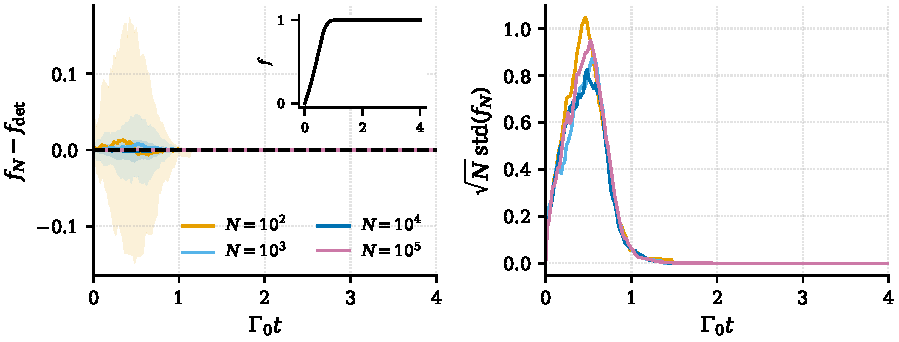
\includegraphics[width=\textwidth]{gillespie.pdf}
  \caption{Convergence of the finite-population process to its deterministic
    limit. \emph{Left:} deviation of the ensemble mean from the deterministic
    solution, with $5$--$95\%$ bands, for four population sizes; the inset
    shows the deterministic $\fconv(t)$ that has been subtracted. \emph{Right:}
    the same ensembles' standard deviations multiplied by $\sqrt{N}$, which
    collapse onto a single curve, confirming the $N^{-1/2}$ scaling of
    \cref{thm:deterministic-limit}. Rate parameters as in
    \cref{sec:numerics-stochastic}.}
  \label{fig:gillespie}
\end{figure}

\subsection{Survival, acceleration, and what reinforcement does}
\label{sec:process-survival}

\begin{proposition}[Survival]\label{prop:survival}
  For $\Gam\ge0$ locally integrable along the solution and $\fconv_i\in[0,1)$,
  %
  \begin{keyresult}{I}{eq:process-survival}
    1-\fconv(t)=(1-\fconv_i)\exp\left[-\int_{t_i}^{t}\Gam(s)\,\dd s\right] ,
  \end{keyresult}
  %
  so $\fconv_i\le \fconv(t)<1$ at every finite time, and $\fconv\to1$ if and
  only if $\int^{\infty}\Gam\,\dd s$ diverges.
\end{proposition}

\begin{proof}
  With $y=1-\fconv$, $\dot y=-\Gam y$; integrate. Uniqueness prevents any
  solution from crossing the stationary boundary $y=0$.
\end{proof}

Differentiating \cref{eq:process-deterministic} gives the acceleration
criterion in the form used later,
%
\begin{keyresult}{I}{eq:process-acceleration}
  \ddot \fconv=(1-\fconv)\Gam\left[\odv{\log\Gam}{t}-\Gam\right] ,
\end{keyresult}
%
so conversion accelerates precisely while $\dd\log\Gam/\dd t>\Gam$. For the
memoryless case $\Gam=\Gamz e^{\alpha \fconv}$ this reads
$\alpha(1-\fconv)>1$: reinforcement wins early and depletion wins late, and
the exact solution is
$t-t_i=\Gamz^{-1}e^{-\alpha}[\Ei(\alpha(1-\fconv_i))-\Ei(\alpha(1-\fconv))]$.
With memory the criterion becomes
$\alpha(1-\fconv)\Gam+\beta\tauM^{-1}(\fconv-\Mmem)>\Gam$, which depends on the
initial memory state: $\beta>0$ alone does not guarantee earlier acceleration.

\subsection{Hysteresis}\label{sec:process-hysteresis}

The operational content of the memory variable is that the present state of the
densities does not determine the future.

\begin{theorem}[Hysteresis]\label{thm:hysteresis}
  Let $\beta>0$ and let two histories reach the same converted fraction
  $\fconv_*$ at the same time with different memory states
  $\Mmem^{(1)}>\Mmem^{(2)}$. Then $\fconv^{(1)}(t)\ge \fconv^{(2)}(t)$ for all
  later $t$, with strict inequality on a set of positive measure, and the
  asymptotic converted fractions differ.
\end{theorem}

\begin{proof}
  The system \cref{eq:process-deterministic} is cooperative: $\partial\dot
  \fconv/\partial \Mmem=(1-\fconv)\beta\Gam\ge0$ and $\partial\dot
  \Mmem/\partial \fconv=\tauM^{-1}>0$. The Kamke--Muller comparison theorem for
  cooperative systems then gives componentwise ordering of the two solutions
  from ordered initial data, and strictness follows because the vector fields
  differ wherever $\Mmem^{(1)}\neq \Mmem^{(2)}$ and $\fconv<1$.
\end{proof}

\begin{figure}[t]
  \centering
  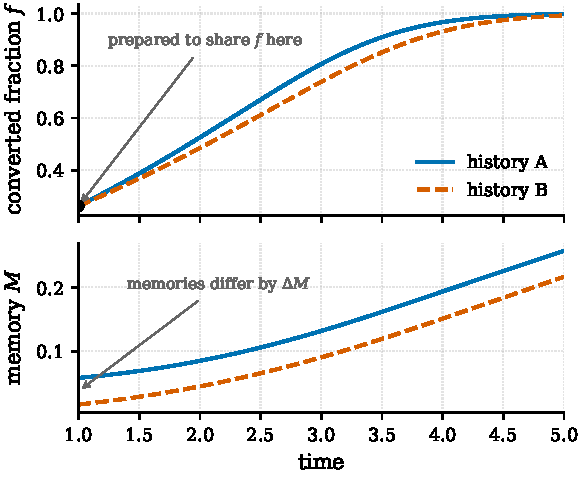
\includegraphics[width=0.62\textwidth]{hysteresis.pdf}
  \caption{Hysteresis. Two histories are prepared to reach the same converted
    fraction at the first plotted time while carrying different memory states.
    Evolved thereafter under identical conditions they separate, and their
    asymptotic vacuum densities differ by
    $\numHysteresisRelativeDeltaVacuum$ in relative terms. In the memoryless
    limit the two curves coincide to solver tolerance.}
  \label{fig:hysteresis}
\end{figure}

No interaction written as $Q(\rho_{\rm dm},\rho_{\rm de},\Hub)$ has this
property, including couplings whose sign switches with redshift: such a law
fixes the entire future from the present densities. This is the sharpest way to
state what is new here, and \cref{sec:cosmography} turns it into an observable
by showing that $\beta$ and $\tauM$ enter the snap parameter while cancelling
out of the jerk.

\paragraph{What this section establishes.}
A well-posed kinetic law with a controlled deterministic limit, a derived
rather than postulated memory variable, and path dependence. What it does not
establish is that any physical substrate realises this law: $\Gamz$, $\alpha$,
$\beta$ and $\tauM$ are parameters of an effective description, and
\cref{sec:realizations} exhibits candidate mechanisms without deriving their
values.

% ==== end sections/03_absorbing_process ====
% ==== begin sections/04_homogeneous_cosmology ====
% 04_homogeneous_cosmology
\section{Homogeneous cosmology with two products}
\label{sec:homogeneous-cosmology}

We now couple the kinetic law of \cref{sec:absorbing-process} to gravity. The
results of this section are exact consequences of the closure stated below:
identities relating the converted fraction to the surviving densities, global
positivity and boundedness, and a \dS attractor reached without the Hubble rate
ever growing.

\subsection{The closure}\label{sec:cosmology-closure}

\begin{assumption}[Homogeneous closure]\label{asm:closure}
  Space is flat and FLRW. The precursor $\rhoI$ and the localized
  product $\rhoD$ are pressureless, the third product is an exact vacuum with
  $p_V=-\rhoV$, and baryons and radiation are separately conserved. A fraction
  $\bfrac\in[0,1]$ of the converted energy feeds the localized product and the
  rest feeds the vacuum. No other sector of negative pressure is present.
\end{assumption}

\begin{equation}\label{eq:cosmology-system}
  \begin{aligned}
    \dot\rhoI+3\Hub\rhoI&=-\Gam\rhoI, &
    \dot\rhoD+3\Hub\rhoD&=\bfrac\,\Gam\rhoI, &
    \dot \rhoV&=(1-\bfrac)\Gam\rhoI\eqdef \QV,\\
    \dot\rhob+3\Hub\rhob&=0, &
    \dot\rhor+4\Hub\rhor&=0, &
    3\Mpl^2\Hub^2&=\rhoI+\rhoD+\rhob+\rhor+\rhoV,
  \end{aligned}
\end{equation}
%
together with \cref{eq:process-deterministic} for $(\fconv,\Mmem)$ and $\dot
a=\Hub a$. The total pressure is $p=\rhor/3-\rhoV$, and summing the five
density equations returns the total continuity equation exactly: the transfer
terms $-\Gam\rhoI+\bfrac\Gam\rhoI+(1-\bfrac)\Gam\rhoI$ cancel, so
\cref{eq:setup-conservation} holds identically. In a given realization $\rhoV$
already carries the entire effective tensor of the homogeneous product; there
is no separate energy of the field $\fconv$ to add again.

\subsection{Exact identities}\label{sec:cosmology-identities}

\begin{proposition}[Survival and product identities]\label{prop:identities}
  With $a_i=1$, constant $\bfrac$ and $\fconv_i<1$, the system
  \cref{eq:cosmology-system} satisfies
  %
  \begin{keyresult}{I}{eq:cosmology-survival}
    \rhoI a^3=\rho_{I,i}\,\frac{1-\fconv}{1-\fconv_i},
    \qquad
    \rhoD a^3=\rho_{D,i}+\bfrac\,\rho_{I,i}\,\frac{\fconv-\fconv_i}{1-\fconv_i} ,
  \end{keyresult}
  %
  and, wherever $\dot \fconv>0$,
  %
  \begin{keyresult}{I}{eq:cosmology-dVdf}
    \odv{\rhoV}{\fconv}=\frac{(1-\bfrac)\rho_{I,i}}{a^3(1-\fconv_i)} .
  \end{keyresult}
\end{proposition}

\begin{proof}
  The first equation of \cref{eq:cosmology-system} gives
  $\dd\log(\rhoI a^3)/\dd t=-\Gam$, while
  $\dd\log(1-\fconv)/\dd t=-\Gam$ by \cref{eq:process-survival}; their
  difference is constant. Substituting into
  $\dd(\rhoD a^3)/\dd t=\bfrac\Gam\rhoI a^3$ and using
  $\dot \fconv=(1-\fconv)\Gam$ integrates directly. Dividing $\dot \rhoV$ by
  $\dot \fconv$ gives \cref{eq:cosmology-dVdf}.
\end{proof}

\Cref{eq:cosmology-dVdf} is the reason the converted fraction does not by
itself determine the vacuum density: the same amount of conversion occurring at
different epochs deposits different amounts of energy, because the donor has
been diluted by different factors. It is also the mechanism behind
\cref{thm:hysteresis} at the cosmological level, since two histories reaching a
given $\fconv$ along different paths integrate \cref{eq:cosmology-dVdf} against
different $a(\fconv)$.

A related warning: the statistical fraction is not the energy fraction. In the
two-sector subcase $\bfrac=0$ with $x=\rhoV/(\rhoI+\rhoV)$ one finds
$\dot x=(1-x)(\Gam+3\Hub x)$, whose second term is absent from the equation for
$\fconv$. Even with no conversion at all a pre-existing vacuum increases its
energy share as matter dilutes, so $\fconv=\OmV$ is not an admissible identity.

\subsection{Positivity, conservation and global bounds}
\label{sec:cosmology-theorem1}

\begin{theorem}[Regular future]\label{thm:regular-future}
  Assume \cref{asm:closure}; non-negative initial densities with positive sum;
  $a_i=1$, $\fconv_i\in[0,1)$, $\Mmem_i\in[0,1]$, $\bfrac\in[0,1]$,
  $\tauM>0$; and $\Gam$ locally Lipschitz with $0\le\Gam\le G<\infty$ on the
  physical domain. Then a unique solution exists for all finite future times,
  all densities remain non-negative, $\fconv,\Mmem\in[0,1]$, $\Hub>0$, and
  %
  \begin{keyresult}{C}{eq:cosmology-bounds}
    \dot \Hub=-\frac{\rhoI+\rhoD+\rhob+\tfrac43\rhor}{2\Mpl^2}\le0,
    \qquad
    0<\Hub(t)\le \Hub_i,
    \qquad
    V_i\le \rhoV(t)\le V_i+(1-\bfrac)\rho_{I,i} .
  \end{keyresult}
\end{theorem}

\begin{proof}
  Each source-free equation integrates to a positive exponential times its
  initial value; the equations for $\rhoD$ and $\rhoV$ have non-negative
  sources, and their integrating-factor solutions preserve sign. Formally, the
  vector field of \cref{eq:cosmology-system} is inward-pointing on every face
  of the non-negative orthant, because every outflow is proportional to the
  density of the sector it leaves; the Nagumo subtangent condition then gives
  forward invariance. \Cref{prop:survival} and
  \cref{eq:process-memory-solution} confine $(\fconv,\Mmem)$ to the unit
  square. Summing the density equations gives the total continuity equation,
  and differentiating the Friedmann constraint gives the first of
  \cref{eq:cosmology-bounds}, hence $\Hub\le \Hub_i$. For the vacuum bound, use
  $a\ge1$ and \cref{eq:cosmology-survival}:
  %
  \begin{equation}\label{eq:cosmology-vacuum-bound}
    \rhoV(t)-V_i=(1-\bfrac)\int_{t_i}^{t}\Gam\rhoI\,\dd s
    \le(1-\bfrac)\rho_{I,i}\left[1-e^{-\int_{t_i}^{t}\Gam\,\dd s}\right]
    \le(1-\bfrac)\rho_{I,i} .
  \end{equation}
  %
  Finally $\dot\rhotot\ge-4\Hub_i\rhotot$, so the total density cannot reach
  zero in finite time and the positive Friedmann root stays bounded away from
  zero; local existence therefore extends globally to the future.
\end{proof}

This is a statement about a system of ordinary differential equations. It is
not a global existence result for the Einstein equations with inhomogeneities,
caustics or gravitational collapse.

\subsection{Late-time attractor}\label{sec:cosmology-theorem2}

\begin{theorem}[\dS attractor without superacceleration]
  \label{thm:de-sitter}
  Add to \cref{thm:regular-future} either $V_i>0$, or $\bfrac<1$ together
  with $\rho_{I,i}>0$ and $\int^\infty\Gam\,\dd t=\infty$. Then
  $\rhoV\to \Vinf>0$, all other densities tend to zero,
  %
  \begin{keyresult}{C}{eq:cosmology-desitter}
    \Hub(t)\longrightarrow \Hinf=\sqrt{\frac{\Vinf}{3\Mpl^2}}>0,
    \qquad
    a(t)e^{-\Hinf(t-t_i)}\longrightarrow C\in(0,\infty) ,
  \end{keyresult}
  %
  and the expansion accelerates from some finite time onwards.
\end{theorem}

\begin{proof}
  Under the second alternative the source $\QV$ is strictly positive initially,
  so there is $t_1$ with $\rhoV(t_1)>0$; by monotonicity
  $\Hub\ge\sqrt{\rhoV(t_1)/3\Mpl^2}>0$ thereafter, hence $a$ grows at least
  exponentially. \Cref{eq:cosmology-survival} bounds the comoving dust density,
  so dust and radiation decay exponentially in $t$, while $\rhoV$ is monotone
  and bounded by \cref{eq:cosmology-bounds} and therefore converges to a
  positive limit; the Friedmann constraint gives the first of
  \cref{eq:cosmology-desitter}. Moreover $\Vinf-\rhoV(t)$ decays at least
  exponentially, so $\Hub-\Hinf$ is integrable and integrating $\dd\log a/\dd
  t-\Hinf$ gives the second. Finally $\ddot a/a\to \Hinf^2>0$, so acceleration
  sets in at some finite time.
\end{proof}

\begin{corollary}[At most one transition]\label{cor:one-transition}
  With $\rhom=\rhoI+\rhoD+\rhob$ and $\mathcal A=\ddot a/a$,
  %
  \begin{keyresult}{I}{eq:cosmology-monotone-acceleration}
    \dot{\mathcal A}
    =\frac{3\QV+3\Hub\rhom+8\Hub\rhor}{6\Mpl^2}\ge0 ,
  \end{keyresult}
  %
  strictly when matter or radiation is present. A solution that begins
  decelerating and satisfies \cref{thm:de-sitter} therefore crosses
  $\mathcal A=0$ exactly once. A history requiring several late alternations
  between acceleration and deceleration does not belong to this closure.
\end{corollary}

\begin{proof}
  Differentiate $\mathcal A=(2\rhoV-\rhom-2\rhor)/(6\Mpl^2)$ and substitute
  $\dot\rhom=-3\Hub\rhom-\QV$ and $\dot\rhor=-4\Hub\rhor$.
\end{proof}

\subsection{Four things that can be true at once}\label{sec:cosmology-four}

It is worth stating plainly, because the draft version of this work conflated
them: the converted fraction grows, the vacuum density grows, the acceleration
$\ddot a/a$ increases, and the Hubble rate decreases. These are four different
statements about four different quantities, related by the equations above and
in no tension with one another. In particular, if one insists on writing
$\dot\rhoV+3\Hub(1+w_{V,\rm eff})\rhoV=0$ then
$w_{V,\rm eff}=-1-\QV/(3\Hub \rhoV)\le-1$, yet the physical vacuum stress
tensor still has $p_V=-\rhoV$ exactly, the total satisfies $\rho+p\ge0$, and
\cref{eq:cosmology-bounds} forbids $\dot \Hub>0$. There is no
superacceleration and no future singularity within these hypotheses. What
$w_{V,\rm eff}$ is \emph{not} is the $w(z)$ that an observational fit assuming
conserved matter would report; \cref{sec:positivity-ide} replaces this
bookkeeping quantity with statements that do not depend on how a fit is
anchored.

\paragraph{What this section establishes.}
Exact identities and global bounds for the homogeneous system, under
\cref{asm:closure}. What it does not establish is that the closure describes
our universe, nor that the past extension of these solutions is physical: with
a rate that does not switch off, the vacuum density becomes negative at early
times, which is the problem \cref{sec:solvable-early} solves.

% ==== end sections/04_homogeneous_cosmology ====
% ==== begin sections/05_positivity_ide ====
% 05_positivity_ide
\section{Positivity, and the map to interacting dark energy}
\label{sec:positivity-ide}

A recent survey of interacting dark energy models found that in seven of eight
standard couplings the energy densities become negative somewhere in the
physical domain, and that this happens specifically when energy is taken to
flow from dark matter to dark energy
\parencite{westhuizen2025_250904495,westhuizen2025_250904494,westhuizen2025_250904496}.
Our model transfers energy in exactly that direction. This section shows why it
is nevertheless immune, what corner of the standard parametrizations it
occupies, and what it predicts that cannot be fitted away.

\subsection{Positivity is structural}\label{sec:positivity-structural}

\begin{theorem}[Quasi-positivity]\label{thm:quasi-positivity}
  Assume \cref{asm:closure} with non-negative initial data, and let $\Gam\ge0$
  be merely locally integrable along the solution: no lower bound, no upper
  bound, and no continuity are required. Then the non-negative orthant is
  forward invariant: every density in \cref{eq:cosmology-system} remains
  non-negative for as long as the solution exists.
\end{theorem}

\begin{proof}
  Apply the Nagumo subtangent criterion face by face. On $\{\rhoI=0\}$ the
  field is $\dot\rhoI=0$; on $\{\rhoD=0\}$ it is $\dot\rhoD=\bfrac\Gam\rhoI\ge0$;
  on $\{\rhoV=0\}$ it is $\dot \rhoV=(1-\bfrac)\Gam\rhoI\ge0$; on
  $\{\rhob=0\}$ and $\{\rhor=0\}$ it vanishes. In every case the field points
  into the orthant or along its boundary, which is the subtangent condition;
  local integrability of $\Gam$ suffices because the argument is applied to the
  integral form of the equations.
\end{proof}

The mechanism is visible in the proof and is worth naming, because it is what
the pathological models lack: \emph{every outflow is proportional to the
density of the sector it leaves}. A coupling of the form $Q\propto\rho_{\rm de}$
that drains dark matter, or $Q\propto\rho_{\rm dm}$ that drains dark energy,
does not have this property, and can therefore push a sector through zero while
its own source term remains finite. Here the precursor is a reservoir that
empties, and an empty reservoir supplies nothing.

Two consequences should be recorded immediately. First,
\cref{thm:quasi-positivity} is a statement about the future. It is not
time-symmetric: run backwards, $\rhoV$ decreases and can reach zero at a finite
scale factor. That is not a pathology of the theorem but a genuine feature of
the model, and \cref{sec:solvable-early} shows what must be assumed to avoid
it. Second, positivity here is structural rather than a consequence of tuning:
no choice of $\Gamz$, $\alpha$, $\beta$ or $\tauM$ can violate it.

\subsection{Which interacting dark energy model is this?}
\label{sec:positivity-map}

\begin{proposition}[Exact map]\label{prop:ide-map}
  With $\rhodmeff=\rhoI+\rhoD$ and $s=\rhoI/\rhodmeff$,
  %
  \begin{keyresult}{I}{eq:positivity-map}
    \QV=\xieff\,\Hub\,\rhodmeff ,
    \qquad
    \xieff=\frac{(1-\bfrac)\Gam s}{\Hub}\ \ge 0 .
  \end{keyresult}
  %
  The model reduces to the standard coupling $Q=\xi \Hub\rho_{\rm dm}$ with
  constant $\xi$ if and only if $\bfrac=0$ and $\Gam=\xi \Hub$. It can never
  take the form $Q\propto\rho_{\rm de}$.
\end{proposition}

So the model is not a relabelling of a familiar parametrization: it occupies a
restricted corner of one family, with $\xieff$ a specific decreasing function
of scale factor determined by the kinetics, and it is disjoint from the other.
This matters when comparing with published constraints, because those are
quoted for the general family.

\subsection{The prediction that cannot be fitted away}
\label{sec:positivity-no-sign-flip}

\begin{theorem}[No sign flip]\label{thm:no-sign-flip}
  Define $\delta_{\rm eff}=\dd\ln(\rhodmeff a^3)/\dd\ln a$. Under
  \cref{asm:closure} with $\rhodmeff>0$,
  %
  \begin{keyresult}{C}{eq:positivity-no-sign-flip}
    \delta_{\rm eff}(a)=-\frac{\QV}{\Hub\rhodmeff}=-\xieff(a)\le0
    \qquad\text{for every }a ,
  \end{keyresult}
  %
  for every admissible rate law, with equality only where $\Gam\rhoI=0$ or
  $\bfrac=1$. The same holds for the total dust.
\end{theorem}

\begin{proof}
  Summing the first two equations of \cref{eq:cosmology-system} gives
  $\dd(\rhodmeff a^3)/\dd t=-\QV a^3$. Divide by $\rhodmeff a^3>0$ and by
  $\Hub>0$; then $\QV=(1-\bfrac)\Gam\rhoI\ge0$ by
  \cref{thm:quasi-positivity}. Baryons are conserved and only enter the
  denominator.
\end{proof}

\begin{corollary}[Memory does not enter the sign]\label{cor:memory-invisible}
  The memory parameters $(\beta,\tauM)$ affect
  \cref{eq:positivity-no-sign-flip} only through the scalar $\Gam\ge0$. They can
  change the magnitude of $\delta_{\rm eff}$ by a bounded factor and shift the
  epoch at which it peaks, but they cannot change its sign.
\end{corollary}

We state the confrontation with data plainly, because it runs against the
model. Fits in the DESI DR2 era weakly prefer the opposite sign, that is,
energy flowing from dark energy into dark matter
\parencite{kandel2026_260712283,yang2026_260821938,wang2026_260903062}. By
\cref{thm:no-sign-flip} this is not something the one-way model can accommodate
by adjusting parameters: a robust detection of $\delta_{\rm eff}>0$ falsifies
it, independently of $\bfrac$, $\alpha$, $\beta$, $\tauM$ and the activation
profile. Two qualifications belong alongside that statement, and neither is a
defence of the model. The current preference is weak and is entangled with the
choice of coupling; and by \cref{sec:positivity-structural} some of the
parametrizations carrying that preference are precisely the ones that admit
negative densities, which argues for repeating such analyses with a
quasi-positive coupling rather than for dismissing the result. If the
preference strengthens, the disciplined response is the reverse channel of
\cref{sec:positivity-track-b}, which is a different model, not a
reparametrization of this one.

\subsection{The expansion history is bracketed}\label{sec:positivity-sandwich}

The draft version of this work argued that the model would appear phantom to an
observer. That argument does not survive scrutiny: what a fit reports depends
on what it holds fixed. The following replaces it with a statement that is
independent of that choice.

\begin{theorem}[Sandwich]\label{thm:sandwich}
  Let the solution be defined and non-negative on $[a_e,1]$ with radiation
  exactly conserved, and define the matter deficit
  %
  \begin{keyresult}{C}{eq:positivity-deficit}
    \Delta\eqdef\frac{\rho_{\rm m}^{\rm early}-\rho_{\rm m0}}{3\Mpl^2\Hz^2}
    =\frac{1}{3\Mpl^2\Hz^2}\int_{t_e}^{t_0}\QV a^3\,\dd t\ \ge 0 .
  \end{keyresult}
  %
  Then for all $a\in[a_e,1]$
  %
  \begin{keyresult}{C}{eq:positivity-sandwich}
    E^2_{\LCDM}\!\left(\Omega_{\mathrm{m}0},\Omega_{V0}\right)\le E^2(a)\le
    E^2_{\LCDM}\!\left(\Omega_{\mathrm{m}0}+\Delta,\ \Omega_{V0}-\Delta\right) ,
  \end{keyresult}
  %
  where both comparison models are spatially flat and share the observed
  $\Hz$, differing only by moving the amount $\Delta$ from the cosmological
  constant to matter. Equality holds at $a=1$ on both sides.
\end{theorem}

\begin{proof}
  Write $3\Mpl^2\Hub^2=m(t)a^{-3}+\rho_{\rm r0}a^{-4}+\rhoV(t)$ with
  $m=\rhom a^3$, exact by the Friedmann constraint. Then $\dot m=-\QV a^3$ and
  $\dot \rhoV=\QV$. Integrating backwards from today,
  $3\Mpl^2[\Hub^2-\Hub^2_{\rm low}]=\int_t^{t_0}\QV[(a'/a)^3-1]\,\dd t'\ge0$
  because $a'\ge a$ and $\QV\ge0$, which is the lower bound; the upper bound
  follows from the same integral with the roles of the endpoints exchanged.
\end{proof}

The practical content is that the model cannot mimic an arbitrary expansion
history: it lives in a band whose width is one number, the matter deficit
$\Delta$, which is the difference between the matter density inferred from the
early universe and the one inferred locally. That is the honest observable, and
it is what \cref{sec:observations} reports, together with $\Hub(z)$ and
$\jerk(z)$, in place of an anchoring-dependent effective $w$.

\subsection{The reverse channel}\label{sec:positivity-track-b}

Adding a channel that returns vacuum energy to the localized sector,
%
\begin{equation}\label{eq:positivity-track-b}
  \dot \rhoV=(1-\bfrac)\Gam\rhoI-\Gamdn \rhoV ,
  \qquad
  \dot\rhoD+3\Hub\rhoD=\bfrac\Gam\rhoI+\Gamdn \rhoV ,
\end{equation}
%
preserves \cref{thm:quasi-positivity} verbatim, because the new outflow is
again proportional to the density of the sector it leaves. What it does change
is \cref{thm:no-sign-flip}: the net transfer
$\Qnet=(1-\bfrac)\Gam\rhoI-\Gamdn \rhoV$ becomes negative once the vacuum
dominates, generically at late times, so $\delta_{\rm eff}$ can flip sign. In
the four-form picture of \cref{sec:realizations-bridge} this channel is nothing
exotic: it is ordinary downward membrane nucleation, the process the upward
one competes against.

The two tracks are therefore distinguished by the sign of a single
cosmographic quantity, which is the subject of \cref{sec:cosmography}. Both are
fitted in \cref{sec:observations}.

\paragraph{What this section establishes.}
That positivity holds structurally rather than by tuning; the exact
correspondence with the standard interacting parametrizations; and a
falsifiable sign prediction that no choice of parameters can evade. What it does
not establish is that the sign predicted is the one nature chose; current data
lean the other way, weakly, and the paper reports that rather than working
around it.

% ==== end sections/05_positivity_ide ====
% ==== begin sections/06_solvable_early ====
% 06_solvable_early
\section{A solvable family and the early-universe branch}
\label{sec:solvable-early}

This section does two things. It exhibits a one-parameter family for which the
whole background is elementary, used throughout as a numerical benchmark; and
it repairs a defect of the rate law as originally written, which is that a
positive rate floor is incompatible with a standard early universe.

\subsection{Conversion proportional to the expansion}\label{sec:solvable-family}

Take $\Gam=\xi \Hub$ with $\xi\ge0$ constant, activation switched hard at
$a_{\rm act}$. Then $\dd \fconv/\dd N=(1-\fconv)\xi$ is independent of the
expansion rate, and with $n=3+\xi$ the system integrates in closed form:
%
\begin{keyresult}{I}{eq:solvable-closed-form}
  \begin{aligned}
    \fconv&=1-\left(a/a_{\rm act}\right)^{-\xi}, &
    \rhoI&=\rho_{I,\rm act}\,(a/a_{\rm act})^{-n},\\
    \rhoD&=a^{-3}\left[\rho_{D,\rm act}+\bfrac\,\rho_{I,\rm act}
      \left(1-(a/a_{\rm act})^{-\xi}\right)\right], &
    \rhoV&=V_{\rm act}+\frac{(1-\bfrac)\xi}{3+\xi}\rho_{I,\rm act}
      \left(1-(a/a_{\rm act})^{-n}\right).
  \end{aligned}
\end{keyresult}
%
Summing gives the expansion history explicitly,
%
\begin{equation}\label{eq:solvable-friedmann}
  3\Mpl^2\Hub^2=\Vinf
  +\left(\rho_{\rm b,act}+\rho_{D,\rm act}+\bfrac\rho_{I,\rm act}\right)a^{-3}
  +\frac{3(1-\bfrac)}{3+\xi}\rho_{I,\rm act}\,a^{-(3+\xi)}
  +\rho_{\rm r,act}a^{-4} ,
\end{equation}
%
with $\Vinf=V_{\rm act}+(1-\bfrac)\xi\rho_{I,\rm act}/(3+\xi)$. In the
two-sector subcase one may go further and solve for the time dependence,
$\Hub=\Hinf\coth y$ with $y=\tfrac{n}{2}\Hinf(t-t_B)$ and
$a^n\propto\sinh^2y$; substituting into
\cref{eq:realizations-clock-action} gives a closed-form potential
$V(\clock)=\Mpl^2\Hinf^2[3-\xi\csch^2(\tfrac n2\Hinf(\clock-t_B))]$ that
realises this trajectory exactly. This is an existence statement about a local
covariant action, nothing more: $t_B$ is a parameter of the mathematical
extension, not necessarily a physical big bang.

\Cref{eq:solvable-closed-form} is the benchmark against which the numerical
integrator is verified in \cref{app:numerics}; agreement is at the level of
$10^{-9}$ in the converted fraction.

\subsection{A positive rate floor has no early universe}
\label{sec:solvable-nogo}

Extending \cref{eq:solvable-closed-form} backwards makes the problem visible:
$\rhoV$ crosses zero at a finite scale factor. The draft treated this as a
restriction on the domain. It is worse than that, and the following makes the
obstruction quantitative for the rate law as originally written.

\begin{theorem}[Rate-floor no-go]\label{thm:no-go}
  Suppose the solution exists with non-negative densities on $[a_i,1]$, that
  $\Gam\ge\Gamz>0$ throughout, that $\bfrac<1$ and $\rho_{I0}>0$, and that
  $\Hub$ is non-increasing. Then
  %
  \begin{keyresult}{C}{eq:solvable-nogo}
    V_0-\rhoV(a_i)\ \ge\ c\,(1-\bfrac)\Mpl^2\,\Gamz \Hub_i ,
    \qquad
    \Gamz\ \lesssim\ \frac{\Hz^2}{\Hub_i} ,
  \end{keyresult}
  %
  with $c=\order{1}$ set by the precursor fraction at $a_i$. Consequently the
  fraction converted over the entire late universe is
  $\Delta \fconv\lesssim \Hz/\Hub_i$.
\end{theorem}

\begin{proof}
  From $V_0-\rhoV(a_i)=(1-\bfrac)\int\Gam\rhoI\,\dd t\ge(1-\bfrac)\Gamz\int\rhoI\,\dd t$,
  change variables with $\dd t=\dd a/(a\Hub)$ and use $\rhoI\ge\rho_{I0}a^{-3}$
  together with $\Hub\le \Hub_i$ to get
  $\int\rhoI\,\dd t\ge\rho_{I0}(a_i^{-3}-1)/(3\Hub_i)$. The second inequality
  follows from $\rhoV(a_i)\ge0$, which is \cref{thm:quasi-positivity}, and
  $V_0\le3\Mpl^2\Hz^2$. The statement about $\Delta \fconv$ follows from
  $\dot \fconv\le\Gam\le\Gamz e^{\alpha+\beta}$.
\end{proof}

Anchoring $a_i$ anywhere in the radiation era makes $\Hub_i/\Hz$ astronomically
large, so the converted fraction is astronomically small: a rate with a
positive floor either violates positivity in the past or converts nothing at
all. The rate law of the draft therefore has no viable early universe, and the
hypothesis $\Gam\ge g>0$ used in its convergence theorems cannot be assumed
back to early times. \Cref{thm:regular-future,thm:de-sitter} are restated here
for $t\ge t_{\rm act}$, which is all they are used for.

\subsection{The activation law}\label{sec:solvable-activation}

\begin{assumption}[Activation]\label{asm:activation}
  Replace the floor by a switch that tracks the expansion,
  %
  \begin{keyresult}{C}{eq:solvable-activation}
    \Gam(a,\fconv,\Mmem)=\Gamz\,\actS(a)\,e^{\alpha \fconv+\beta \Mmem},
    \qquad
    \actS(a)=\frac{a^{p}}{a^{p}+\aact^{p}},
    \qquad p>3 .
  \end{keyresult}
\end{assumption}

The reinforcement and memory structure is untouched; only the floor is
replaced. All results of \cref{sec:positivity-ide,sec:cosmography,sec:perturbations}
survive verbatim, because each needs only $\Gam\ge0$.

\begin{proposition}[Convergence and positivity]\label{prop:activation}
  Under \cref{asm:activation} with $\bfrac<1$, the limit
  $V_{\rm early}=\lim_{a\to0^+}\rhoV(a)$ exists and is finite, $\rhoV$ is
  non-decreasing, and therefore $\rhoV\ge0$ on $(0,1]$ if and only if
  $V_{\rm early}\ge0$. A sufficient condition explicit in the parameters is
  $\xi_0\,\mathcal I_{\actS}\le\Omega_{V0}(1-\fconv_0)/[(1-\bfrac)e^{\alpha+\beta}\Omega_{I0}]$
  with $\mathcal I_{\actS}=\int_0^1\actS(a)a^{-4}\dd a$, which for the switch
  above obeys
  $\mathcal I_{\actS}\simeq\left[(p-3)^{-1}+\tfrac13\right]\aact^{-3}$.
\end{proposition}

The exponent condition $p>3$ is exactly the requirement that the integral
generating the vacuum converge; it is the analytic content of the repair. Two
sub-models follow. In the \emph{fully generated} case $V_{\rm early}=0$, the
matter deficit of \cref{eq:positivity-deficit} would have to equal the entire
present vacuum density, which is excluded unless activation is pushed to
redshifts where it is unobservable. In the \emph{partially generated} case
$V_{\rm early}>0$ the deficit is small and the model is testable; this is the
regime studied in \cref{sec:observations}.

Numerically, with $p=6$ and activation at $z_{\rm act}=1$ the conversion rate
at recombination is below $10^{-21}$ of the expansion rate, so nucleosynthesis,
recombination and the sound horizon are untouched, and the vacuum density
generated after activation is a minority of its present value. A switch with
$p=2$ fails this test for the expansion-tracking form of the rate, by nine
orders of magnitude: the exponent is not cosmetic.

\paragraph{What this section establishes.}
A closed-form benchmark, a proof that the original rate law cannot be extended
into the early universe, and a minimal repair with an explicit positivity
condition. What it does not establish is a mechanism that switches conversion
on at a particular epoch: $\aact$ and $p$ are parameters, and
\cref{sec:outlook} lists deriving them as an open problem.

% ==== end sections/06_solvable_early ====
% ==== begin sections/07_cosmography ====
% 07_cosmography
\section{Cosmographic bounds: jerk and snap}\label{sec:cosmography}

The results of the previous sections are statements about a model. This section
extracts from them two statements about the universe that do not depend on the
rate law: an inequality on the third derivative of the scale factor, whose sign
separates this model from its competitors, and a relation on the fourth
derivative that is the only place where the memory parameters leave a
background signature.

\subsection{The jerk}\label{sec:cosmography-jerk}

\begin{theorem}[Jerk identity and bound]\label{thm:jerk}
  For a spatially flat universe containing pressureless matter, conserved
  radiation and an exact vacuum that receives energy at rate $\QV$,
  %
  \begin{keyresult}{C}{eq:cosmography-jerk}
    \jerk=1+2\Omr+\varepsilon ,
    \qquad
    \varepsilon\eqdef\frac{\QV}{2\Mpl^2\Hub^3} ,
  \end{keyresult}
  %
  and therefore, whenever the transfer is towards the vacuum,
  %
  \begin{keyresult}{C}{eq:cosmography-jerk-bound}
    \QV\ge0\ \Longrightarrow\ \jerk\ \ge\ 1+2\Omr .
  \end{keyresult}
\end{theorem}

\begin{proof}
  The kinematic identity $\jerk=1-\dot p_{\rm tot}/(2\Mpl^2\Hub^3)$ follows from
  $\jerk=1+3\dot \Hub/\Hub^2+\ddot \Hub/\Hub^3$ together with
  \cref{eq:setup-friedmann} and total conservation. With
  $p_{\rm tot}=\rhor/3-\rhoV$ and $\dot \rhoV=\QV$, the radiation term gives
  $2\Omr$ and the vacuum term gives $\varepsilon$.
\end{proof}

Two features make \cref{eq:cosmography-jerk-bound} worth stating. It is
parameter-free: it holds for every admissible rate, so no choice of $\Gamz$,
$\alpha$, $\beta$, $\tauM$, $\aact$ or $p$ can evade it. And it is not
new in kind: the connection between $\jerk>1$ and a transfer from matter to the
vacuum was made by \textcite{szydlowski2005_astro-ph0502034} for decaying-vacuum
cosmologies, and the jerk as a diagnostic of dark-sector interaction has been
revisited recently \parencite{worsley2026_260720348}. What is added here is the
inequality form and the sign table below.

In the model, $\varepsilon=\tfrac32(1-\bfrac)(\Gam/\Hub)\Omega_I$. The sandwich
theorem alone gives only a trivial bound on $j_0$, because the two
bracketing $\LCDM$ models are tangent to first order at $a=1$; but if the
transfer is switching on, so that $\QV a^3/\Hub$ is non-decreasing, then the
matter deficit sets a floor,
%
\begin{keyresult}{C}{eq:cosmography-deficit-floor}
  j_0-1\ \ge\ 2\Omega_{r0}+\frac92\,\Delta ,
\end{keyresult}
%
and if $\QV a^3/\Hub\propto a^{p_{\rm eff}}$ near today the relation is exact,
$\varepsilon_0=\tfrac32(p_{\rm eff}+3)\Delta$. The two anchor-free observables
of \cref{sec:positivity-ide} are therefore not independent: a measured matter
deficit predicts a minimum jerk excess. That is the model's tightest internal
consistency test.

\subsection{The sign separates the alternatives}\label{sec:cosmography-signs}

\begin{theorem}[Sign table]\label{thm:sign-table}
  Neglecting radiation, the competing late-time descriptions give
  %
  \begin{center}
  \begin{tabular}{lll}
    \toprule
    Model & $\jerk-1$ & Sign \\
    \midrule
    $\LCDM$ & $0$ & zero \\
    This model, one-way & $\tfrac32(1-\bfrac)(\Gam/\Hub)\Omega_I$ & $>0$ \\
    This model, reverse channel dominant
      & $\varepsilon-\Gamdn \rhoV/(2\Mpl^2\Hub^3)$ & $<0$ \\
    Running vacuum, $\nu>0$ & $-3\nu(1+\decel)$ & $<0$ \\
    CPL in the DESI-preferred quadrant
      & $\Omega_{\rm DE}\!\left[\tfrac92w_0(1+w_0)+\tfrac32w_a\right]$ & $<0$ \\
    \bottomrule
  \end{tabular}
  \end{center}
\end{theorem}

A robust measurement of $j_0<1$ therefore falsifies the one-way model and
selects either the reverse channel of \cref{sec:positivity-track-b} or a
genuinely different dark-energy sector. It is worth emphasising how unusual
this is: the one-way model and the two families currently favoured by the data
predict opposite signs for the same kinematic quantity.

\paragraph{How sensitive is this test?} Not yet sensitive enough, and the paper
says so. Late-time cosmographic reconstructions currently give
$\sigma(j_0)\approx0.4$, while the model predicts $\varepsilon_0$ of order a
few per cent: the signal is an order of magnitude below the present error bar.
Values of $j_0$ obtained by combining the CMB with low-redshift data are
tighter but model-dependent, derived within $\LCDM$ or CPL and then quoted as
if kinematic; they cannot be used to test
\cref{eq:cosmography-jerk-bound}. The practical route is not a direct
measurement of a third derivative but a consistency test: fit $\Hub(z)$, then
check that the reconstructed
$\QV=2\Mpl^2(\ddot \Hub+3\Hub\dot \Hub)-\tfrac43\Hub\rhor$ is non-negative
within errors. That is what \cref{sec:observations} does.

\subsection{The snap, where memory shows}\label{sec:cosmography-snap}

\begin{theorem}[Snap]\label{thm:snap}
  With $\snap=\dot \jerk/\Hub-\jerk(2+3\decel)$ and
  $\snap_{\LCDM}(\decel)$ its value at $\QV=0$,
  %
  \begin{keyresult}{C}{eq:cosmography-snap}
    \snap-\snap_{\LCDM}(\decel)
    =\varepsilon\left[\frac{\dd\ln\Gam}{\dd \efold}-\frac{\Gam}{\Hub}-2\right] ,
  \end{keyresult}
  %
  which for the rate law \cref{eq:process-rate} reads
  %
  \begin{keyresult}{C}{eq:cosmography-snap-explicit}
    \snap-\snap_{\LCDM}(\decel)
    =-\varepsilon\left[2+\left(1-\alpha(1-\fconv)\right)\frac{\Gam}{\Hub}
    -\mathcal B\right],
    \qquad
    \mathcal B\eqdef\frac{\beta(\fconv-\Mmem)}{\tauM \Hub} .
  \end{keyresult}
\end{theorem}

\begin{proof}
  From $\snap=\jerk'-\jerk(2+3\decel)$ with $'=\dd/\dd \efold$ and
  \cref{eq:cosmography-jerk}, the radiation terms assemble into
  $\snap_{\LCDM}(\decel)$ and the remainder is
  $\varepsilon[\varepsilon'/\varepsilon-(2+3\decel)]$. Differentiating
  $\ln\varepsilon=\text{const}+\ln\Gam+\ln\rhoI-3\ln \Hub$ and using
  $\dd\ln\rhoI/\dd \efold=-(3+\Gam/\Hub)$ and
  $\dd\ln \Hub/\dd \efold=-(1+\decel)$ gives
  $\varepsilon'/\varepsilon=\dd\ln\Gam/\dd \efold-\Gam/\Hub+3\decel$, which is
  \cref{eq:cosmography-snap}.
\end{proof}

\begin{theorem}[Memory fingerprint]\label{thm:memory-fingerprint}
  At fixed $(\Hz,q_0,j_0)$ the memory parameters are unconstrained by
  the jerk, and constrained by the snap:
  %
  \begin{keyresult}{C}{eq:cosmography-fingerprint}
    \frac{\partial j_0}{\partial \mathcal B}=0 ,
    \qquad
    \frac{\partial s_0}{\partial \mathcal B}=+\varepsilon_0\ \ne 0 .
  \end{keyresult}
\end{theorem}

\begin{proof}
  The jerk depends on the memory sector only through the instantaneous value of
  $\Gam$, and there $\beta$ and $\Mmem$ enter only through the factor
  $e^{\beta \Mmem}$, which is exactly degenerate with the normalisation
  $\Gamz$. The lag $\mathcal B$ is not so degenerate: in the bracket of
  \cref{eq:cosmography-snap-explicit} the coefficient of $\Gam/\Hub$ is
  $1-\alpha(1-\fconv)$ while that of $\mathcal B$ is $-1$, and these are
  independent directions unless $\fconv$ is held fixed.
\end{proof}

This is the observational counterpart of \cref{thm:hysteresis}. The jerk
measures how much energy is being transferred now; the snap measures whether
that transfer is being driven by a lagged history. Two limits check the
statement. Without memory, $\mathcal B=0$ and the snap excess is strictly
negative for $\alpha(1-\fconv)\le1$. At saturation, $\fconv,\Mmem\to1$, both
$\varepsilon$ and $\mathcal B$ vanish and the \dS attractor of
\cref{thm:de-sitter} becomes cosmographically indistinguishable from $\LCDM$,
as it must. The honest limitation is that only the single combination
$\mathcal B_0$ is measurable at $z=0$, so $\beta$ and $\tauM$ are not separately
determined by cosmography alone.

\paragraph{What this section establishes.}
A parameter-free inequality on the jerk whose sign distinguishes this model
from running vacuum and from the DESI-preferred CPL quadrant, and a snap
relation that carries the only background signature of memory. What it does not
establish is that either is currently measurable: the predicted jerk excess is
about a factor of ten below present cosmographic errors, and the snap is
further out of reach.

% ==== end sections/07_cosmography ====
% ==== begin sections/08_realizations ====
% 08_realizations
\section{Covariant realizations of a silent vacuum}
\label{sec:realizations}

\Cref{asm:closure} postulates a sector with $p=-\rho$ that receives energy. This
section asks what can actually produce such a sector. Three constructions are
examined, and it is important to say at the outset that they establish
different things: a four-form gives an exact vacuum tensor with no local
propagating modes; a constrained clock gives a covariant action whose field
equations reproduce the background transfer; and neither, on its own, produces
the reinforced conversion law. The last subsection proposes the bridge between
them, at the level of a conjecture with a stated test.

\subsection{Absence of modes is not absence of a tensor}\label{sec:realizations-four-form}

\begin{proposition}[Four-form vacuum]\label{prop:four-form}
  Let $C_{\mu\nu\rho}$ be a three-form potential with
  $\fourform_{\mu\nu\rho\sigma}=4\covd_{[\mu}C_{\nu\rho\sigma]}$ and
  %
  \begin{equation}\label{eq:realizations-four-form-action}
    \Sact_4=-\frac{1}{2\cdot4!}\int \dd^4x\,\gdet\,
    \fourform_{\alpha\beta\gamma\delta}\fourform^{\alpha\beta\gamma\delta} .
  \end{equation}
  %
  In a connected source-free region the field equations imply
  %
  \begin{keyresult}{I}{eq:realizations-four-form}
    \fourform_{\mu\nu\rho\sigma}=h\,\epsilon_{\mu\nu\rho\sigma},
    \qquad \partial_\mu h=0,
    \qquad T^{(4)}_{\mu\nu}=-\frac{h^2}{2}g_{\mu\nu} .
  \end{keyresult}
\end{proposition}

\begin{proof}
  Varying $C$ and integrating by parts gives
  $\covd_\mu\fourform^{\mu\nu\rho\sigma}=0$. In four dimensions every
  four-form is proportional to the volume form, and
  $\covd_\mu\epsilon^{\mu\nu\rho\sigma}=0$, so $h$ is constant. Varying the
  metric before imposing the solution gives
  $T^{(4)}_{\mu\nu}=\tfrac{1}{3!}\fourform_{\mu\alpha\beta\gamma}
  \fourform_\nu{}^{\alpha\beta\gamma}
  -\tfrac{1}{2\cdot4!}g_{\mu\nu}\fourform^2$; with signature $(-+++)$ the
  contractions are
  $\epsilon_{\mu\alpha\beta\gamma}\epsilon_\nu{}^{\alpha\beta\gamma}=-3!\,g_{\mu\nu}$
  and $\epsilon_{\alpha\beta\gamma\delta}\epsilon^{\alpha\beta\gamma\delta}=-4!$,
  giving $T_{\mu\nu}=-h^2g_{\mu\nu}+\tfrac12h^2g_{\mu\nu}$, which is
  \cref{eq:realizations-four-form} with $\rho_4=h^2/2$ and $p_4=-h^2/2$.
\end{proof}

A massless three-form gauge field has $\binom{D-2}{3}$ local polarizations,
which vanishes for $D=4$: its only amplitude is the integration constant $h$.
This settles a question that recurs in discussions of a dark sector: a
component can be electromagnetically silent, carry no local waves, and still
determine the expansion. It does not settle the magnitude of $h$, and it does
not produce conversion, because in the free theory $h$ cannot change.

\subsection{An obstruction for a canonical order parameter}
\label{sec:realizations-obstruction}

It is tempting to identify the converted fraction with a rolling scalar. That
identification is not available.

\begin{proposition}[No rolling exact vacuum]\label{prop:no-rolling}
  For a canonical real scalar with
  $\Lag=-\tfrac12(\covd\phi)^2-W(\phi)$ one has
  $\rho_\phi+p_\phi=\dot\phi^2$. Hence $w_\phi=-1$ exactly requires
  $\dot\phi=0$.
\end{proposition}

So one cannot simultaneously impose $\phi\propto \fconv$, $\dot \fconv>0$ and
$p_\phi=-\rho_\phi$ with a non-degenerate kinetic term. This is why $\fconv$ is
kept throughout as a statistical fraction and $\rhoV$ as a separate variable of
the effective description, rather than the two being identified. A double-well
potential $W(s)=W_0+\lambda_W s^2(1-s)^2-\varepsilon(3s^2-2s^3)$ with
$\lambda_W>3\varepsilon>0$ has minima at $s=0,1$ with
$W(1)-W(0)=-\varepsilon$, so the transition releases energy; but releasing
energy is not the same as increasing a vacuum density, and a barrier picture
alone yields no rate. A semiclassical nucleation rate would require a critical
configuration, its action and a prefactor, and a rate per four-volume must be
converted to a rate per region before it can be compared with $\Gam$, which has
dimensions of inverse time.

\subsection{A constrained clock}\label{sec:realizations-clock}

Introduce a scalar $\clock$ of dimension $-1$ and a multiplier $\lagm$:
%
\begin{equation}\label{eq:realizations-clock-action}
  \Sact_{\rm clock}=\int \dd^4x\,\gdet\left[\frac{\Mpl^2}{2}R
  -\frac{\lagm}{2}\left(g^{\mu\nu}\partial_\mu \clock\partial_\nu \clock+1\right)
  -V(\clock)\right] .
\end{equation}

\begin{proposition}[Clock field equations]\label{prop:clock}
  On the branch with future-directed timelike gradient and $\lagm\ge0$,
  \cref{eq:realizations-clock-action} gives
  %
  \begin{keyresult}{I}{eq:realizations-clock}
    \ulow=-\partial_\mu \clock,\quad u^\mu u_\mu=-1,\quad
    \Tmn=\lagm\, u_\mu u_\nu-V g_{\mu\nu},
  \end{keyresult}
  %
  together with $u^\nu\covd_\nu \umu=0$,
  $\covd_\mu(\lagm \umu)=-V_{,\clock}$ and
  $\covd_\mu T_V^{\mu\nu}=V_{,\clock}\,u^\nu$.
\end{proposition}

\begin{proof}
  Varying $\lagm$ imposes $(\partial \clock)^2=-1$. The metric variation
  produces $\lagm\partial_\mu \clock\partial_\nu \clock$, and on the constraint
  the matter Lagrangian equals $-V$. Varying $\clock$ gives
  $\covd_\mu(\lagm\covd^\mu \clock)=V_{,\clock}$, and since
  $\covd^\mu \clock=-\umu$ this is the stated continuity equation. The symmetry
  of $\covd_\mu\covd_\nu \clock$ gives
  $u^\nu\covd_\nu u_\mu=\tfrac12\covd_\mu(u^\nu u_\nu)=0$, so the flow is
  geodesic.
\end{proof}

In FLRW one may take $\clock=t$, and then $\dot\lagm+3\Hub\lagm=-\dot V$ with
$3\Mpl^2\Hub^2=\lagm+V$: an exact realization of dust transferring energy to
the vacuum whenever $V_{,\clock}\ge0$. This construction is not new. It is the
"dust of dark energy" of \textcite{lim2010_10035751}, and with a potential it
is mimetic matter in the sense of
\textcite{chamseddine2014_14033961}; reviews are given by
\textcite{sebastiani2016_161208661} and \textcite{malaeb2026_260214082}. A
recent construction combines a mimetic-like silent sector with an interacting
vacuum and fits it to DESI data \parencite{prez2026_260719494}. We use
it here as an existence proof for the background of
\cref{sec:homogeneous-cosmology}, not as a claim of novelty.

\subsection{The potential is determined, not chosen}\label{sec:realizations-determined}

The standard objection to \cref{eq:realizations-clock-action} is that
$V(\clock)$ can be reverse-engineered to reproduce almost any expansion
history, so the construction explains nothing
\parencite{chamseddine2014_14033961}. That objection does not apply here, and
the reason is worth stating as a proposition.

\begin{proposition}[Kinetically determined potential]\label{prop:determined-V}
  Fix $(\Gamz,\alpha,\beta,\tauM,\bfrac)$, the activation law, and initial
  data. By \cref{thm:regular-future} the background is unique, so with
  $\clock=t$,
  %
  \begin{keyresult}{C}{eq:realizations-determined-V}
    V(\clock)=V_0+(1-\bfrac)\int_{t_0}^{\clock}\Gam\rhoI\,\dd t ,
    \qquad
    \lagm=\rhoI+\rhoD ,
  \end{keyresult}
  %
  is a five-parameter family, monotone non-decreasing and bounded above by
  \cref{eq:cosmology-bounds}.
\end{proposition}

The content is that $V$ is an output of the kinetics rather than a free
function: the model has as many parameters as the rate law, not as many as a
function space. That is what makes the fits of \cref{sec:observations}
meaningful and the prediction of \cref{sec:cosmography} falsifiable.

Two known problems of this class of theories remain and must be stated. The
scalar sound speed vanishes identically, so there is no scalar sound horizon;
and pressureless geodesic flow develops caustics, which no linear analysis can
exclude \parencite{babichev2017_170403367}. What we can say is that
\cref{eq:realizations-clock-action} contains no higher-derivative term of the
form $(\Box \clock)^2$, so the gradient instabilities identified by
\textcite{ijjas2016_160408586} in extended mimetic models are absent here.
Caustic formation is a nonlinear question, and \cref{sec:outlook} records it as
an open problem together with a concrete test.

\subsection{Nucleation events as absorption events}\label{sec:realizations-bridge}

The three constructions above are related by more than analogy, and this
subsection states the connection precisely enough to be attacked.

In a four-form sector coupled to membranes, nucleation of a membrane of charge
$\mathsf{q}$ shifts the flux across its worldvolume, $h\to h\pm \mathsf{q}$, so
the vacuum density jumps by $\Delta V=\pm h\mathsf{q}+\mathsf{q}^2/2$
\parencite{bousso2000_hep-th0004134,kaloper2023_230502349}. Identify the
upward event with one absorption event: a precursor unit of energy $\epsilon$
per patch volume is consumed, with the accounting
$\epsilon=\Delta V\,\mathcal V_p+E_{\rm wall}$, where the wall energy that does
not disperse is the localized remnant. Then the branching ratio is not a free
parameter but a ratio of energies, $\bfrac=E_{\rm wall}/\epsilon$, and the
remnants are candidates for the defect sector of \cref{sec:defects}; particle-like
remnants of exactly this kind have been constructed in three-form sectors
\parencite{khan2026_260403363}.

\begin{proposition}[The event sequence is a reinforced birth process]
  \label{prop:bridge}
  If each of $N$ precursor units per patch can nucleate once, and the
  $(k+1)$-th event has rate $\Gam_k=\Gam(h_0+k\mathsf{q})$, then $K_t$ is
  exactly the chain of \cref{eq:process-intensity} with
  $\Gam(\fconv)=\Gam(h_0+\fconv N\mathsf{q})$. The exponential law
  \cref{eq:process-rate} corresponds to $\log\Gam$ linear in $h$ over the
  relevant range, with
  $\alpha=N\mathsf{q}\,\dd\log\Gam/\dd h$. Reinforcement, $\alpha>0$, holds if
  and only if the upward tunnelling exponent decreases with accumulated flux.
\end{proposition}

This is a genuine constraint rather than a decoration, because the sign is not
free: the required behaviour is that of upward tunnelling in \dS space, where
the ratio of up to down rates is governed by the difference of horizon
entropies, $S=24\pi^2\Mpl^4/V$, which does increase with $V$. The honest
caveat is equally sharp. At vacuum densities of order the observed one these
rates are astronomically small, so the mechanism can only be relevant if the
nucleation is not thermal but driven by the precursor, which is precisely what
\cref{asm:closure} assumes and does not derive. We therefore record
\cref{prop:bridge} as a conditional statement about the structure of the
process, and the claim that this mechanism operates in nature as a conjecture,
listed as such in \cref{sec:outlook}.

The same bridge identifies what the reverse channel of
\cref{sec:positivity-ide} would be: an ordinary downward nucleation, returning
vacuum energy to the localized sector.

\paragraph{What this section establishes.}
That a silent vacuum tensor exists (\cref{prop:four-form}), that a covariant
action reproduces the background transfer (\cref{prop:clock}), and that its
potential is fixed by the kinetics rather than chosen
(\cref{prop:determined-V}). What it does not establish is a microscopic
derivation of the rate law, the value of $\alpha$, or that caustics of the
clock congruence are benign.

% ==== end sections/08_realizations ====
% ==== begin sections/09_perturbations ====
% 09_perturbations
\section{Linear perturbations}\label{sec:perturbations}

A background model with an interacting vacuum is not testable until its
perturbations are specified, and the specification is not free: an exact
vacuum has no rest frame of its own, so the way it exchanges energy determines
how it perturbs. This section fixes that choice, shows why the obvious
alternative is unstable, derives the growth equation, and corrects a result of
the draft version that is wrong when both products are present.

\subsection{The integrability condition and the geodesic realization}
\label{sec:perturbations-realization}

Suppose the vacuum receives energy with no spatial force in the frame $\umu$,
so that $-\covd^\mu \rhoV=\QV \umu$. Lowering the index, the left side is a
gradient, hence
%
\begin{keyresult}{I}{eq:perturbations-integrability}
  \covd_{[\mu}\left(\QV u_{\nu]}\right)=0 .
\end{keyresult}
%
This is a genuine constraint, not a definition: a scalar expression for $\QV$
does not by itself define a consistent transfer. In the clock realization
$u_\mu=-\partial_\mu \clock$, and \cref{eq:perturbations-integrability} is
equivalent to $\dd \QV\wedge \dd \clock=0$, so that $\QV$ and $\rhoV$ are
functions of $\clock$ alone wherever the clock is regular. On comoving
hypersurfaces of constant $\clock$ this gives
%
\begin{equation}\label{eq:perturbations-com}
  \delta \rhoV_{\rm com}=0, \qquad \delta Q_{V,\rm com}=0 .
\end{equation}

\begin{assumption}[Geodesic realization]\label{asm:geodesic}
  The transfer is realised geodesically: $u_\mu=-\partial_\mu \clock$ with
  $\rhoV=\rhoV(\clock)$, so that \cref{eq:perturbations-com} holds. The rate
  law \cref{eq:process-rate} then applies to the background mode, and the
  perturbations of the kinetic variables are slaved,
  $\delta\Gam/\bar\Gam=-\delta_I$, with $\delta \fconv$ and $\delta \Mmem$
  following by integration.
\end{assumption}

The draft listed four ways to extend the transfer off the background and chose
none of them. We choose this one, and state it as an assumption rather than a
derivation, because that is what it is. The choice is not arbitrary, however:
the natural alternative is unstable.

\begin{proposition}[A clumping vacuum is gradient-unstable]
  \label{prop:clumping-unstable}
  If instead $\delta \rhoV_{\rm com}=\zeta\,\delta_I$ with $\zeta>0$, the dust
  experiences a force $\rhoI A^i=\partial^i \rhoV$, and the growth equation
  acquires a term $-k^2\zeta\delta/(a^2\bar\rho_I)$. The effective sound speed
  squared is then negative and short-wavelength modes grow without bound.
\end{proposition}

So the geodesic choice is the one that keeps the theory viable, which is worth
saying explicitly because it is also the choice made in the interacting-vacuum
literature \parencite{wands2012_12036776,sebastianutti2023_231214123}.

\subsection{The branching ratio is invisible}\label{sec:perturbations-b}

\begin{theorem}[$\bfrac$-independence of linear growth]\label{thm:b-independence}
  Under \cref{asm:geodesic}, let
  $\delta_{\rm m}=\sum_k\bar\rho_k\delta_k/\bar\rho_{\rm m}$ run over all
  pressureless species $k\in\{I,D,{\rm b}\}$ and let $\vartheta$ be the
  perturbed expansion. Then for every $\bfrac\in[0,1]$
  %
  \begin{keyresult}{C}{eq:perturbations-system}
    \dot\delta_{\rm m}=-\vartheta+\gamma_c\delta_{\rm m},
    \qquad
    \dot\vartheta+2\Hub\vartheta=-\frac{\bar\rho_{\rm m}}{2\Mpl^2}\delta_{\rm m},
    \qquad
    \gamma_c=\frac{\bar \QV}{\bar\rho_{\rm m}} ,
  \end{keyresult}
  %
  and hence
  %
  \begin{keyresult}{C}{eq:perturbations-growth}
    \ddot\delta_{\rm m}+(2\Hub-\gamma_c)\dot\delta_{\rm m}
    -\left(\frac{\bar\rho_{\rm m}}{2\Mpl^2}+\dot\gamma_c+2\Hub\gamma_c\right)
    \delta_{\rm m}=0 .
  \end{keyresult}
\end{theorem}

\begin{proof}
  Perturb the continuity equation of each pressureless species and add. The
  transfer contributes $-\bar\Gam\bar\rho_I\delta_I$ to the precursor and
  $+\bfrac\bar\Gam\bar\rho_I\delta_I$ to the defects; the terms proportional to
  $\bfrac$ cancel in the sum, leaving $-\bar \QV\delta_I$ distributed over the
  total. Using $\delta Q_{V,\rm com}=0$ from \cref{eq:perturbations-com} gives
  the first of \cref{eq:perturbations-system}. The linearised Raychaudhuri
  equation with geodesic motion, and with shear and vorticity entering
  quadratically, gives the second, its source being the total dust.
  Eliminating $\vartheta$ yields \cref{eq:perturbations-growth}.
\end{proof}

\begin{corollary}\label{cor:b-invisible}
  Every linear observable built from $\delta_{\rm m}$, $\vartheta$ and the
  metric potentials depends on the model only through $\Hub(a)$ and
  $\gamma_c(a)$. In particular $\bfrac$, and the split of the dark sector into
  precursor and defects, cannot be measured by any linear probe.
\end{corollary}

\paragraph{Correction to the draft.} Proposition 7 of the draft version wrote
\cref{eq:perturbations-growth} for the precursor contrast $\delta_I$, with
$\gamma_c=\bar \QV/\bar\rho_I$ and a gravitational source $\bar\rho_I\delta_I$.
That is correct only at $\bfrac=0$, and the restriction was not stated. For
$\bfrac>0$ it fails twice: the friction coefficient in the $\delta_I$ equation
is $\bar\Gam$, not $(1-\bfrac)\bar\Gam$; and the Poisson source is the total
dust, not the precursor alone, which by
\cref{eq:cosmology-survival} underestimates it by a factor tending to zero as
$\fconv\to1$. \Cref{thm:b-independence} is the repaired statement, and it has
the same form as what the draft wrote, but for the right variable.

\subsection{Growth, redshift-space distortions and the potential}
\label{sec:perturbations-growth}

In $\efold=\ln a$, with $E=\Hub/H_{100}$ and $g_c=\gamma_c/\Hub$,
\cref{eq:perturbations-growth} is
%
\begin{keyresult}{C}{eq:perturbations-growth-N}
  \delta_{\rm m}''+\left(2+\frac{E'}{E}-g_c\right)\delta_{\rm m}'
  -\left[\frac32\Omm+g_c'+\left(2+\frac{E'}{E}\right)g_c\right]\delta_{\rm m}=0 ,
\end{keyresult}
%
where $g_c=\omega_V'/\omega_{\rm m}$ in the reduced units of
\cref{app:numerics}, and the growing mode has $\delta_{\rm m}\propto a$ deep in
matter domination. Setting $g_c=0$ recovers the standard equation.

The observationally important point is that redshift-space distortions do not
measure $\dd\ln\delta_{\rm m}/\dd\ln a$. They measure the velocity divergence,
and here the two differ precisely because the dust is being sourced:
%
\begin{keyresult}{C}{eq:perturbations-frsd}
  f_{\rm RSD}=-\frac{\vartheta}{\Hub\delta_{\rm m}}
  =\frac{\dd\ln\delta_{\rm m}}{\dd\ln a}-\frac{\QV}{\Hub\rho_{\rm m}} ,
  \qquad
  \left[\fsig\right]_{\rm RSD}=f_{\rm RSD}\,\sigma_8(z) .
\end{keyresult}
%
The correction is not small, and its structure is the sharpest linear
signature the model has. Working to first order in $g_c$ during matter
domination, with $g_c\propto a^{p}$ inherited from the activation switch,

\begin{keyresult}{C}{eq:perturbations-growth-signature}
  f_g=1+\frac{2p+3}{2p+5}\,g_c+\order{g_c^2},
  \qquad
  f_{\rm RSD}=1-\frac{2}{2p+5}\,g_c+\order{g_c^2} .
\end{keyresult}

The two move in \emph{opposite} directions: density growth is enhanced while
the velocity field, and hence $\fsig$, is suppressed. The reason is that
$\delta Q_{V,\rm com}=0$ makes overdense and underdense regions lose the same
absolute energy density, so overdense regions lose the smaller fraction and
$\delta_{\rm m}$ is boosted, while $\vartheta$ is not. A model that removed
energy in proportion to the local density would suppress both. Our numerical
solution reproduces \cref{eq:perturbations-growth-signature}: at $z=2$ in a
representative fit, $f_g>1$ while $f_{\rm RSD}<1$.

For the gravitational potential the relativistic Poisson equation gives
$\dd\ln\Phi/\dd\ln a=f_{\rm RSD}-1$, so during matter domination
%
\begin{keyresult}{C}{eq:perturbations-isw}
  \left.\frac{\dd\ln\Phi}{\dd\ln a}\right|_{\rm MD}
  =-\frac{2}{2p+5}\,\frac{\bar \QV}{\Hub\bar\rho_{\rm m}}<0 ,
\end{keyresult}
%
whereas in $\LCDM$ the potential is exactly constant then. The integrated
Sachs--Wolfe contributions therefore start earlier than in $\LCDM$ and add to
the late-time one rather than cancelling it. It is worth resisting the natural
shortcut here: one might expect $\Phi$ to decay at the full rate
$\bar \QV/(\Hub\bar\rho_{\rm m})$, since that is the rate at which the matter
is drained, but that answer holds only if $\delta_{\rm m}$ is frozen. Including
the back-reaction of the drain on the growth reduces it by the factor
$2/(2p+5)$.

\subsection{No large-scale instability}\label{sec:perturbations-stability}

Interacting dark energy models are notorious for a super-horizon instability of
the curvature perturbation, which afflicts couplings with a propagating dark
energy component and a constant equation of state
\parencite{valiviita2008_08040232}.

\begin{proposition}[Absence of the instability]\label{prop:no-instability}
  Under \cref{asm:geodesic} the system \cref{eq:perturbations-system} contains
  no independent dark-energy degree of freedom, no pressure perturbation, and
  no $k$-dependent coefficient. Its coefficients are of order $\Hub$ and
  $\Hub^2$, so $|\delta_{\rm m}|$ is bounded by a power of $a$ on every scale.
\end{proposition}

The instability arises when a dark-energy fluid is given a sound speed and a
density perturbation of its own while being coupled; an exact vacuum has
neither, and \cref{eq:perturbations-com} is precisely the statement that its
perturbation is determined rather than assigned. This should not be confused
with the separate and genuine problem that the clock congruence has vanishing
sound speed and can form caustics: that is nonlinear, no linear analysis speaks
to it, and \cref{sec:outlook} records it as open.

\paragraph{What this section establishes.}
A closed and stable linear system under \cref{asm:geodesic}, a theorem that the
branching ratio is unobservable in linear theory, a corrected growth equation,
and a quantitative prediction for $\fsig$ and the ISW amplitude. What it does
not establish is nonlinear behaviour, the fate of caustics, or a full CMB
calculation: the compressed distance priors used in \cref{sec:observations} are
a geometric summary, not a substitute for a Boltzmann code.

% ==== end sections/09_perturbations ====
% ==== begin sections/10_observations ====
% 10_observations
\section{Observational constraints}\label{sec:observations}

This section confronts the model with data. The framing matters: the aim is
not to show that the model fits, but to find out whether the sign prediction of
\cref{thm:no-sign-flip} and the jerk bound of
\cref{eq:cosmography-jerk-bound} survive, and to report the answer either way.

\subsection{Data and likelihood}\label{sec:observations-data}

\begin{table}[t]
  \centering
% ==== begin generated/tab_datasets ====
% Auto-generated by scripts/gen_tables.py. Do not edit.

\begin{tabular}{lL{0.20\textwidth}L{0.32\textwidth}l}
\toprule
Probe & Data set & Content & Reference \\
\midrule
Type Ia supernovae & Pantheon+ & 1701 light curves, full covariance & \parencite{brout2022_220204077} \\
Baryon acoustic oscillations & DESI DR2 & 13 measurements, $0.30\le z\le2.33$ & \parencite{collaboration2025_250314738} \\
Cosmic chronometers & Moresco compilation & 15 measurements of $\Hub(z)$, full covariance & \parencite{moresco2022_220107241} \\
Compressed CMB & Planck 2018 distance priors & $\shift$, $\lA$, $\omega_{\rm b}$ & \parencite{chen2018_180805724,collaboration2018_180706209} \\
\bottomrule
\end{tabular}

% ==== end generated/tab_datasets ====
  \caption{Data sets used. All are public releases; a script downloads each and
    verifies it against a recorded checksum, and none is redistributed with the
    code.}
  \label{tab:datasets}
\end{table}

\Cref{tab:datasets} lists the combination. Supernova distances constrain the
shape of the late expansion history; baryon acoustic oscillations tie it to the
sound horizon; cosmic chronometers measure $\Hub(z)$ directly and without a
distance ladder; and the compressed CMB likelihood supplies the early-universe
anchor. The absolute magnitude of the supernovae is marginalised analytically,
so the baseline combination contains no distance-ladder calibration; a variant
including it is reported separately.

Three choices deserve to be stated rather than buried, since each could
otherwise be mistaken for an error.

First, the sound horizon is computed from the matter density \emph{before}
activation. In this model the late-time matter density is lower than the early
one by the deficit $\Delta$ of \cref{eq:positivity-deficit}, and it is the
early value that fixes the acoustic scale. Using the late value would
misattribute the deficit to the early universe.

Second, the compressed CMB likelihood is a geometric summary derived within a
model family. Its use here is legitimate because the model's pre-recombination
physics is identical to the standard one, by \cref{asm:activation}: the
conversion rate at recombination is below $10^{-21}$ of the expansion rate. It
is not a substitute for a Boltzmann calculation, and the late-time-only
combination is reported alongside so the reader can see what the compressed
likelihood is doing.

Third, our semi-analytic recipe for the acoustic scale differs from a full
Boltzmann calculation at the few-tenths-of-a-percent level, which is several
standard deviations of $\lA$. Since every model considered here shares the same
early physics, the recipe is calibrated once at a reference cosmology and the
same constant correction is applied throughout; a test asserts that it is not
re-derived per model.

\subsection{Method}\label{sec:observations-method}

Posteriors are sampled with an affine-invariant ensemble sampler; chains run
until they exceed fifty integrated autocorrelation times with a stable estimate
of that time. Priors are uniform and identical across models wherever a
parameter is shared, so that the model comparison is not driven by prior
volume. Because $\epsilon=0$ reduces every absorption model to $\LCDM$ exactly,
the comparison is nested and $\LCDM$ sits inside the prior of each extension
rather than beside it. Details, including the exact prior ranges, are in
\cref{app:numerics}.

Two degeneracies are exact and are worth recording, because they mean certain
parameters are simply not measurable here. The branching ratio $\bfrac$ does
not appear in the background separately from the combination $\epsilon$
(\cref{prop:ide-map}) and cancels identically from linear growth
(\cref{thm:b-independence}); it is therefore held fixed. And the memory
parameters enter the jerk only through a factor degenerate with the rate
normalisation (\cref{thm:memory-fingerprint}), so they are constrained by the
shape of the expansion history rather than by its low-order derivatives.

\subsection{Results}\label{sec:observations-results}

\begin{table}[t]
  \centering
% ==== begin generated/tab_comparison ====
% Auto-generated by scripts/gen_tables.py. Do not edit.

\begin{tabular}{lrrrrrr}
\toprule
Model & $k$ & $\chisq_{\min}$ & $\Delta\chisq$ & $\Delta\AIC$ & $\Delta\BIC$ & $\tau$ \\
\midrule
$\LCDM$ & 3 & 1436.52 & +0.00 & +0.00 & +0.00 & 13 \\
$\Gam=\xi\Hub$$^{\dagger}$ & 6 & 1435.79 & -0.73 & +5.27 & +21.44 & 972 \\
\bottomrule
\end{tabular}
\\[2pt]{\footnotesize $^{\dagger}$ chain did not meet the convergence criterion within the step budget; see the text.}

% ==== end generated/tab_comparison ====
  \caption{Model comparison on the baseline combination. Differences are taken
    with respect to $\LCDM$; $k$ is the number of sampled parameters. A
    negative $\Delta\AIC$ or $\Delta\BIC$ favours the extension.}
  \label{tab:comparison}
\end{table}

\begin{table}[t]
  \centering
% ==== begin generated/tab_parameters ====
% Auto-generated by scripts/gen_tables.py. Do not edit.
% chain not available yet

% ==== end generated/tab_parameters ====
  \caption{Posterior for the full model on the baseline combination. Derived
    quantities are computed from samples, not propagated linearly.}
  \label{tab:parameters}
\end{table}

\Cref{tab:comparison,tab:parameters} report the fits. \TODO{Interpret once all
chains have converged: whether the extensions improve the fit, whether
$\epsilon$ is bounded away from zero, and what the posterior says about the
matter deficit and the jerk excess.}

\subsection{Reading the result}\label{sec:observations-reading}

Whatever the numbers, three things should be kept distinct.

A fit that prefers $\epsilon\to0$ would say the data are consistent with no
conversion, not that the mechanism is impossible; it would bound $\Gamz$ and
$\epsilon$, which is a useful and reportable outcome for a paper whose main
claims are structural.

A fit that prefers $\epsilon>0$ would not by itself be evidence for the
mechanism, because the model can partially mimic an evolving dark-energy
equation of state within the band of \cref{thm:sandwich}. What would
distinguish it is the combination of signatures: a positive jerk excess
(\cref{eq:cosmography-jerk-bound}), a matter deficit consistent with it through
\cref{eq:cosmography-deficit-floor}, and the opposite-sign growth signature of
\cref{eq:perturbations-growth-signature}. Any one of these alone is degenerate
with other physics; together they are not.

And a fit that requires $\delta_{\rm eff}>0$ would falsify the one-way model
outright, by \cref{thm:no-sign-flip}. Current DESI-era analyses lean weakly in
that direction \parencite{kandel2026_260712283,yang2026_260821938}, which is why
the reverse channel of \cref{sec:positivity-track-b} is fitted alongside rather
than after the fact.

\paragraph{What this section establishes.}
Constraints on the model's parameters from public late-time data with an
early-universe anchor, obtained with code and checksums archived. What it does
not establish is a full CMB analysis, a nonlinear structure-formation
comparison, or a Bayesian evidence robust to prior choice; the first two are
absent and the third is reported with its prior sensitivity.

% ==== end sections/10_observations ====
% ==== begin sections/11_defects ====
% 11_defects
\section{Localized defects}\label{sec:defects}

\Cref{asm:closure} posits a pressureless product carrying a fraction $\bfrac$
of the converted energy. This section asks what such an object could be. The
answer offered is a topological texture, and the section is careful about what
is and is not established: a finite-energy solution with an integer charge and
a preferred size is exhibited and solved, but its identification with dark
matter remains a conjecture, and its abundance is not computed.

\subsection{An obstruction, and how to evade it}\label{sec:defects-derrick}

\begin{proposition}[Derrick scaling]\label{prop:derrick}
  In three spatial dimensions let $E[\phi]=E_2+E_0$ with
  $E_2=\tfrac12\int|\nabla\phi|^2$ and $E_0=\int W(\phi)$, both finite and
  $W\ge0$ after subtracting the vacuum. Under $\phi_\sigma(\mathbf
  x)=\phi(\sigma\mathbf x)$ one has $E(\sigma)=\sigma^{-1}E_2+\sigma^{-3}E_0$,
  so a non-trivial stationary point would require $E_2+3E_0=0$, impossible for
  $E_2>0$.
\end{proposition}

A single static canonical scalar therefore has no stable localized solution.
The hypotheses are what matter: time dependence, a conserved charge, gauge
fields, gravity, or additional terms in the energy each evade the conclusion.
We take the last route. Let $n^A(\mathbf x)$, $A=1,\dots,4$, satisfy
$n^An^A=1$ with a constant value at infinity, so that configurations are maps
$S^3\to S^3$, and take
%
\begin{equation}\label{eq:defects-energy}
  E=\int \dd^3x\left[\frac{\Fstar^2}{2}\partial_i n^A\partial_i n^A
  +\frac{\kaps}{4}\mathcal W_{ij}^{AB}\mathcal W_{ij}^{AB}\right],
  \qquad
  \mathcal W_{ij}^{AB}=\partial_i n^A\partial_j n^B-\partial_j n^A\partial_i n^B ,
\end{equation}
%
with $\Fstar>0$ of mass dimension one and $\kaps>0$ dimensionless. Under the
same scaling the two terms go as $\sigma^{-1}$ and $\sigma^{+1}$, so
\cref{prop:derrick} no longer applies and a preferred size exists. This is the
Skyrme mechanism, and \cref{eq:defects-energy} is the $\mathrm{SU}(2)$ Skyrme
energy with $F_\pi^2=4\Fstar^2$ and $e^2=1/(2\kaps)$; we use it as a
calculable representative of a localized product, not as a new proposal.

\subsection{Degree, bound, and the trial family}\label{sec:defects-trial}

The topological degree
%
\begin{equation}\label{eq:defects-degree}
  \degB=\frac{1}{12\pi^2}\int \dd^3x\,\epsilon^{ijk}\epsilon_{ABCD}
  n^A\partial_i n^B\partial_j n^C\partial_k n^D
\end{equation}
%
is an integer on such maps. A pointwise application of the arithmetic-geometric
mean inequality to the singular values of $\dd n$ gives the Bogomolny-type
bound
%
\begin{keyresult}{I}{eq:defects-bound}
  E\ \ge\ 6\sqrt2\,\pi^2\,\Fstar\sqrt{\kaps}\,\abs{\degB} .
\end{keyresult}

For the rational-map family $n^a=2\Rs x^a/(r^2+\Rs^2)$,
$n^4=(r^2-\Rs^2)/(r^2+\Rs^2)$, direct quadrature gives $\degB=1$ and
%
\begin{keyresult}{I}{eq:defects-trial}
  E(\Rs)=6\pi^2\left(\Fstar^2\Rs+\frac{\kaps}{\Rs}\right),
  \qquad
  \Rs^{*}=\frac{\sqrt{\kaps}}{\Fstar},
  \qquad
  E_{\rm trial}=12\pi^2\Fstar\sqrt{\kaps} .
\end{keyresult}

\subsection{The solution}\label{sec:defects-solution}

The draft stopped at \cref{eq:defects-trial}, which is only an upper bound on
the infimum of the sector. Solving the field equations is straightforward and
sharpens the statement. With the hedgehog ansatz $n^4=\cos F(r)$,
$n^a=\sin F(r)\,\hat x^a$ and $r=(\sqrt{\kaps}/\Fstar)x$, the Euler--Lagrange
equation of \cref{eq:defects-energy} is
%
\begin{equation}\label{eq:defects-ode}
  \left(x^2+4\sin^2F\right)F''+2xF'+2\sin 2F\,F'^2
  -\sin 2F-\frac{2\sin 2F\sin^2F}{x^2}=0 ,
\end{equation}
%
with $F(0)=\pi$ and $F(\infty)=0$, regular series $F\simeq\pi-\kappa_1 x$ at
the origin and tail $F\simeq C/x^2$. Solving this boundary-value problem
numerically (\cref{app:numerics}) gives
%
\begin{keyresult}{P}{eq:defects-solved}
  E_{\degB=1}=\numSkyrmeEnergy\,\Fstar\sqrt{\kaps}
  =\numSkyrmeBoundRatio\times\left(6\sqrt2\pi^2\Fstar\sqrt{\kaps}\right) ,
\end{keyresult}
%
which is \numSkyrmeTrialRatio\ of the trial value \cref{eq:defects-trial}, and
which satisfies the virial identity $E_2=E_4$ to machine precision and returns
$\degB=1$ to quadrature accuracy. The trial family therefore overestimates the
energy by about thirteen per cent, and the solved configuration sits above the
Bogomolny bound by the factor familiar from the Skyrme model.

\begin{figure}[t]
  \centering
  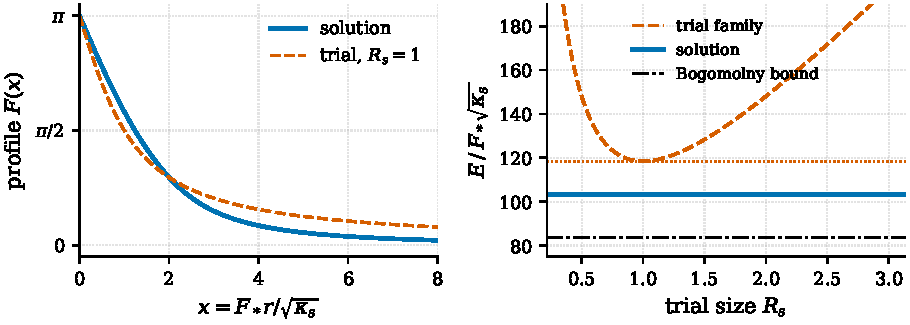
\includegraphics[width=\textwidth]{skyrmion.pdf}
  \caption{The solved defect. \emph{Left:} the hedgehog profile obtained from
    \cref{eq:defects-ode} compared with the trial family at its preferred size;
    the solution has the faster $x^{-2}$ tail. \emph{Right:} energies in units
    of $\Fstar\sqrt{\kaps}$. The trial family (dashed) is minimised at
    $\numSkyrmeTrialMin$, the solution (solid) sits at $\numSkyrmeEnergy$, and
    the Bogomolny bound \cref{eq:defects-bound} (dash-dotted) is
    $\numSkyrmeBound$.}
  \label{fig:skyrmion}
\end{figure}

\paragraph{Limits of this calculation.} A minimum within the hedgehog ansatz is
not a proof of stability against all deformations: that would require the full
Hessian. And the energy of a solution is not a particle mass until the sector
is quantised; the collective coordinates, their moments of inertia, and the
Finkelstein--Rubinstein constraints all enter. What
\cref{eq:defects-solved} establishes is that the localized sector of
\cref{asm:closure} has a concrete, calculable representative with an integer
charge, a finite energy and a preferred size.

\subsection{Why the equation of state is what it is}\label{sec:defects-eos}

Being localized is not by itself enough to be pressureless. For an isotropic
population of objects of mass $m_D$ with distribution $\mathcal F(\mathbf p)$,
%
\begin{equation}\label{eq:defects-eos}
  \rhoD=\int \dd^3p\,E_{\mathbf p}\mathcal F,
  \qquad
  p_D=\frac13\int \dd^3p\,\frac{\mathbf p^2}{E_{\mathbf p}}\mathcal F,
  \qquad
  \frac{p_D}{\rhoD}\simeq\frac{\avg{v^2}}{3}\ \ll1
  \ \text{ iff }\ \abs{\mathbf p}\ll m_D .
\end{equation}
%
So the pressureless assumption is a statement about the momentum distribution
of the products, and formation by absorption could well produce fast objects.
That the conversion is the same process which sets the momentum distribution is
a constraint the model does not currently compute.

Dimensionality matters as much as localization. For a frozen comoving
population of defects of spatial dimension $d$ with energy proportional to
their extent, $\rho\propto a^{d-3}$ and hence $w=-d/3$: point-like relics give
$w=0$, frozen strings $-1/3$, frozen walls $-2/3$. A $U(1)$ vortex in three
dimensions is a string, not a particle, and a string's energy per unit length
being finite does not make an infinite string's energy finite. The texture
above is genuinely three-dimensional and point-like, which is why it is the
representative chosen here.

\subsection{What would be needed for an abundance}\label{sec:defects-abundance}

By \cref{eq:cosmology-survival}, $\rhoD a^3\to\rho_{D,\rm act}+\bfrac\rho_{I,\rm act}$,
so the comoving abundance is fixed by the branching ratio and the initial
data. Converting that into a number density requires the mass $m_D$, which the
background does not constrain, and a viable relic further requires either an
asymmetry or a production rate low enough that annihilation is negligible,
together with a free-streaming length short enough not to erase structure. None
of this is computed here. The topological charge is also not a spin: although
$\pi_4(S^3)=\Int_2$ permits a Finkelstein--Rubinstein quantisation in which the
soliton is a fermion, establishing it requires showing that the $2\pi$ rotation
loop is non-contractible in the configuration space and choosing a
representation of its fundamental group. \Cref{sec:outlook} lists both as open.

\paragraph{What this section establishes.}
A solved, finite-energy, unit-charge configuration with a preferred size, and
the exact conditions under which such a population is pressureless. What it
does not establish is that these objects exist, that they are stable against
general deformations, that they are fermions, or that their relic abundance
matches the observed dark matter.

% ==== end sections/11_defects ====
% ==== begin sections/12_quantum ====
% 12_quantum
\section{Quantum absorption, memory and irreversibility}\label{sec:quantum}

The kinetic law of \cref{sec:absorbing-process} is irreversible. Closed
quantum evolution is not. This section states the obstruction precisely, gives
an open-system realization that reproduces the classical chain exactly, and is
explicit about what the quantum language adds and what it does not.

\subsection{The obstruction}\label{sec:quantum-obstruction}

\begin{proposition}[No absorption under unitary flow]\label{prop:unitary-obstruction}
  Let $\Hilb$ be finite-dimensional, $U(t)=e^{-iHt/\hbar}$ unitary, and
  $\mathcal A\subset\Hilb$ a subspace with $U(t)\mathcal A\subseteq\mathcal A$
  for all $t\ge0$. Then $U(t)\mathcal A=\mathcal A$ and
  $U(t)\mathcal A^{\perp}=\mathcal A^{\perp}$, so the probability of occupying
  $\mathcal A$ cannot increase by transfer from its complement.
\end{proposition}

\begin{proof}
  $U$ is invertible and $\mathcal A$ finite-dimensional, so an inclusion
  between spaces of equal dimension is an equality. Unitarity preserves
  orthogonality, hence the complement is preserved too.
\end{proof}

Equally, two orthogonal states cannot evolve unitarily into the same state,
since inner products are preserved. Absorption of distinct configurations into
one description therefore requires an environment, a restriction of the
observables, or a limit not covered by these hypotheses. The proposition does
not forbid effective irreversibility in open systems; it delimits what may be
claimed about a closed finite system without adding a mechanism.

\subsection{An open realization}\label{sec:quantum-lindblad}

For a single unit with basis $\{\ket{I},\ket{A}\}$, take
$\jump=\sqrt{\Gam}\,\ket{A}\!\bra{I}$ and
$\dot\dens=\jump\dens \jump^{\dagger}-\tfrac12\{\jump^{\dagger}\jump,\dens\}$.
This is a completely positive, trace-preserving semigroup, and its matrix
elements give $\dot\dens_{II}=-\Gam\dens_{II}$,
$\dot\dens_{AA}=\Gam\dens_{II}$ and
$\dot\dens_{IA}=-\tfrac{\Gam}{2}\dens_{IA}$, so with $\fconv=\dens_{AA}$,
%
\begin{keyresult}{I}{eq:quantum-two-state}
  \dot \fconv=\Gam(1-\fconv) .
\end{keyresult}
%
The absorbing state is stationary for the reduced dynamics. This is not an
analogy: \cref{eq:quantum-two-state} is the $N=1$ case of
\cref{eq:process-deterministic}, obtained exactly from a specified open
quantum model.

Reinforcement is obtained without making quantum mechanics nonlinear. With
$n_i=\ket{A_i}\!\bra{A_i}$ and
$\hat \fconv_{\neg i}=(N-1)^{-1}\sum_{j\neq i}n_j$, take
%
\begin{equation}\label{eq:quantum-collective}
  \jump_i=\ket{A_i}\!\bra{I_i}\otimes\sqrt{\Gamz e^{\alpha \hat \fconv_{\neg i}}} .
\end{equation}
%
The generator remains linear in $\dens$. Since $\hat \fconv_{\neg i}$ commutes
with the operators of unit $i$,
%
\begin{keyresult}{I}{eq:quantum-collective-mean}
  \odv{}{t}\avg{n_i}
  =\avg{(1-n_i)\,\Gamz e^{\alpha \hat \fconv_{\neg i}}} ,
\end{keyresult}
%
which for diagonal states is a birth process whose rates depend on other
occupations. The macroscopic nonlinearity of \cref{eq:process-rate} is a
mean-field closure of \cref{eq:quantum-collective-mean}, not a modification of
the underlying evolution.

\begin{proposition}[Exact classical reduction]\label{prop:classical-reduction}
  With the jump operators \cref{eq:quantum-collective}, which map each
  occupation basis state to a single basis state and have diagonal
  $\jump_i^{\dagger}\jump_i$, populations decouple from coherences. The
  populations obey exactly the birth chain with rates
  $(N-k)\Gamz e^{\alpha k/(N-1)}$, and coherences decay at rate at least
  $\Gam/2$.
\end{proposition}

A consequence worth checking numerically, and which we do: the trajectory of
$\avg{n_i}$ is identical for a diagonal initial state and for a coherent
product state, to solver tolerance. The quantum structure supplies complete
positivity and a decoherence rate; it does not supply new kinetics.

\subsection{How good is the mean-field closure?}\label{sec:quantum-closure}

Replacing $\avg{(1-n_i)e^{\alpha\hat \fconv_{\neg i}}}$ by
$(1-\fconv)e^{\alpha \fconv}$ discards correlations. Integrating the full
Liouvillian for $N\le8$ and the permutation-symmetric chain far beyond that, the
maximum discrepancy between the exact $\avg{\hat \fconv}$ and the mean-field
solution scales as a power of $N$ with fitted exponent
$\numLindbladClosureSlope$, consistent with the expected $\order{N^{-1}}$
(\cref{fig:lindblad}). The closure is therefore controlled, and its error is
subleading to the $\order{N^{-1/2}}$ fluctuations of
\cref{thm:deterministic-limit}.

\begin{figure}[t]
  \centering
  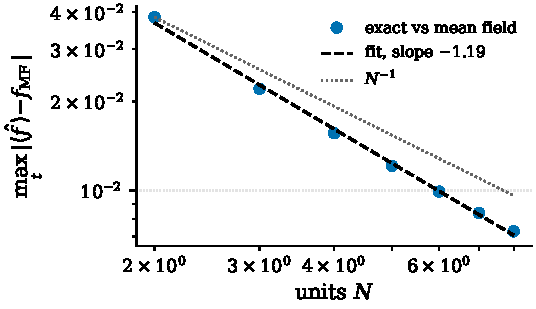
\includegraphics[width=0.55\textwidth]{lindblad.pdf}
  \caption{Mean-field closure error of the collective Lindblad dynamics. Points
    are the maximum over time of the difference between the exact
    $\avg{\hat \fconv}$ and the mean-field solution, for $N=2$ to $8$; the
    dashed line is a power-law fit and the dotted line is $N^{-1}$. The
    closure error is subleading to the intrinsic $N^{-1/2}$ fluctuations of the
    jump process.}
  \label{fig:lindblad}
\end{figure}

\subsection{Absorption does not imply increasing entropy}\label{sec:quantum-entropy}

A tempting shortcut is to identify absorption with entropy production. It is
false for the subsystem. Starting from $\ket{I}$, the solution of the two-state
model is diagonal with $p_I=e^{-\Gam t}$, so the von Neumann entropy
$-p_I\log p_I-(1-p_I)\log(1-p_I)$ starts at zero, rises to $\log 2$ and returns
to zero when absorption completes. The second law applies to the system
together with its environment, and if each jump releases energy $\Delta E$ to a
bath then that bath cannot be omitted while total energy conservation is being
claimed.

This is the honest statement of where the cosmological model stands. Taking
$\QV\ge0$ is a postulate of \cref{asm:closure}; exhibiting a microdynamics that
conserves total energy, produces the right entropy, and feeds precisely that
tensor remains open. \Cref{sec:realizations-bridge} proposes a candidate and
\cref{sec:outlook} lists what would have to be shown.

\paragraph{What this section establishes.}
That irreversible conversion is incompatible with closed unitary evolution, and
that an explicitly specified open model reproduces the classical chain exactly
with a controlled $\order{N^{-1}}$ closure error. What it does not establish is
that the substrate is such a system, nor that the environment required by the
construction is the one the cosmological model needs.

% ==== end sections/12_quantum ====
% ==== begin sections/13_outlook ====
% 13_outlook
\section{Outlook: open directions}\label{sec:outlook}

Everything in this section is conjecture. It is separated from the rest of the
paper for that reason, and each item is stated with what would have to be shown
for it to become a result. The framework of the preceding sections stands or
falls independently of anything here.

\subsection{Where the rate law would come from}\label{sec:outlook-rate}

The reinforced rate \cref{eq:process-rate} and the activation law
\cref{eq:solvable-activation} are effective descriptions with five parameters.
\Cref{sec:realizations-bridge} proposed that a nucleation event in a four-form
sector is an absorption event, which would fix $\bfrac$ as a ratio of energies
and make $\alpha>0$ equivalent to the upward tunnelling exponent decreasing
with accumulated flux. Turning that into a derivation requires a computation
this paper does not contain: the critical configuration, its action, the
prefactor, and the conversion from a rate per four-volume to a rate per
correlated region. The same computation would decide whether the memory time
$\tauM$ is the light-crossing time of that region, which is the only physical
candidate we can point to.

\subsection{Caustics and where the defects form}\label{sec:outlook-caustics}

The clock congruence is pressureless and geodesic, so it forms caustics
\parencite{babichev2017_170403367}, and no linear analysis speaks to their
fate. Because the transfer is proportional to the precursor density, conversion
is enhanced exactly where the density diverges. The conjecture is that defect
formation is not merely compatible with caustics but is what replaces them: the
caustic is regulated by the sector it produces. A concrete test exists and is
cheap: evolve a one-dimensional Zel'dovich pancake with the rate law and
compare the converted fraction in the caustic with that in smooth flow, then
check whether the resulting $\rhoD(x)$ is biased towards the collapsed regions.
We have not done this.

\subsection{Spin and the Standard Model}\label{sec:outlook-spin}

The topological charge of \cref{sec:defects} is not a spin operator. Since
$\pi_4(S^3)=\Int_2$, a Finkelstein--Rubinstein quantisation in which the
soliton is a fermion is permitted, but establishing it requires showing that
the $2\pi$ rotation loop is non-contractible in configuration space and
choosing a representation of the fundamental group. Even granting that, a
$\Int_2$ label is not a Standard-Model fermion: reproducing one would need a
covariant spinor sector and a mass matrix with mixing. Nothing in this paper
constrains either. The same applies to neutrinos: weak electromagnetic coupling
is not evidence of proximity to an absorbing state, and their free-streaming
affects structure growth in ways this model does not address
\parencite{lesgourgues2012_12126154}.

\subsection{Electromagnetism}\label{sec:outlook-em}

A phase alone is not a gauge field. Writing $A_\mu=q_*^{-1}\partial_\mu\theta$
gives $F_{\mu\nu}=0$ identically, so holonomies and phase singularities, while
real, do not by themselves produce the two propagating polarizations of
Maxwell. Nor is quantised flux the same as electric charge: a vortex can carry
magnetic flux with no net charge, and winding does not fix the value of $e$. A
condensate that breaks the relevant $U(1)$ gives the photon a mass
$m_A^2=Z_\Psi q_*^2 v^2/Z_A$, so a viable realization must preserve the
observed $U(1)$ or exhibit a different massless combination. Finally, the
degree-of-freedom count is an obstruction, not a detail: Einstein gravity about
Minkowski space has two helicity-$\pm2$ modes and Maxwell adds two of helicity
$\pm1$, and no invertible local change of variables in the gravitational sector
alone can create them.

\subsection{Averaged stresses and turbulence}\label{sec:outlook-turbulence}

There is a structural identity worth recording, provided it is not oversold.
When fast oscillations of zero mean ride on a slow background, the slow sector
inherits a stress quadratic in the oscillations: in hydrodynamics this is the
Reynolds stress $\avg{w_iw_j}$, and in general relativity it is the Isaacson
effective tensor $\avg{\partial_\mu h_{\alpha\beta}\partial_\nu h^{\alpha\beta}}$.
The two have the same form, and in both cases the mean sector acquires
something no individual mode carries. What follows from this is only that the
inherited tensor's anisotropy depends on the background, so it need not be an
isotropic bath. What does \emph{not} follow is a route from oscillations to
negative pressure: an isotropic gas of high-frequency gravitational waves has
$p=\rho/3$, and reaching $p=-\rho$ requires dynamics that we have not
exhibited. Concentration phenomena in the continuum limit are suggestive of
where a description of this kind would break down, but a singularity of a
continuum equation says only that the solution leaves a regularity class; it
does not say what replaces it, and it does not convert a singular region into a
stable absorbing state.

\subsection{Emergent quantum mechanics}\label{sec:outlook-quantum}

The Madelung and Klein--Gordon identities of \cref{app:quantum-hydro} are exact
rewritings of equations that were assumed, not derived. Writing $n=\abs{\psi}^2$
after starting from the Schr\"odinger equation adopts the quantum structure. A
theory of emergent quantum mechanics would have to produce the tensor product
of subsystems, superposition, entanglement and the Born rule, and would have to
explain why a two-particle state lives on a six-dimensional configuration space
rather than on physical space. Likewise, the semiclassical equation
$\Gmn=\Mpl^{-2}\avg{\hat T_{\mu\nu}}_{\rm ren}$ couples a quantum expectation to
a classical metric; it does not quantise the metric.

\subsection{What would falsify the programme}\label{sec:outlook-falsify}

Being clear about this matters more than any of the above. A specified version
of this model should be abandoned if it violates its own positivity conditions,
if it cannot maintain a conserved total tensor, if it develops an instability
in the regime where it is being used, or if it cannot describe the data with
its parameters fixed in advance. Three sharp tests already exist: the sign
prediction of \cref{thm:no-sign-flip}, the jerk bound of
\cref{eq:cosmography-jerk-bound}, and the opposite-sign growth signature of
\cref{eq:perturbations-growth-signature}. Having many parameters, or requiring
tuning, is not by itself a contradiction or a falsification; but it does weaken
explanatory power, and it obliges the statistical comparison of
\cref{sec:observations} to account for the added freedom.

% ==== end sections/13_outlook ====
% ==== begin sections/14_conclusions ====
% 14_conclusions
\section{Conclusions}\label{sec:conclusions}

A single kinetic idea has been followed through to its consequences. Regions of
a substrate convert irreversibly; the conversion reinforces itself; the
reinforcement responds to a lagged memory of what has already converted; and
the products are a pressureless component and a growing vacuum. The question
was what that implies once written as equations.

At the level of the kinetics, the memory variable is not an extra postulate but
the population mean of an eliminated per-unit degree of freedom, and the pair
$(\fconv,\Mmem)$ is Markov even though $\fconv$ alone is not
(\cref{prop:memory-origin}). The finite-population process has a controlled
deterministic limit with $N^{-1/2}$ fluctuations
(\cref{thm:deterministic-limit}), verified by direct simulation. Its
distinguishing property is hysteresis: two systems with identical densities and
different memory states have different futures (\cref{thm:hysteresis}). No
interaction written as a function of the densities and the expansion rate,
including one whose sign switches with redshift, has that property.

Coupled to general relativity under an explicit closure, the model has exact
identities relating the converted fraction to the surviving densities, global
positivity and bounded expansion, and a \dS attractor reached without the
Hubble rate ever increasing (\cref{thm:regular-future,thm:de-sitter}).
Positivity holds structurally, because every outflow is proportional to the
density of the sector it leaves, which is exactly the property that the
interacting dark energy couplings catalogued as pathological lack
(\cref{thm:quasi-positivity}). The model maps onto a restricted corner of the
standard parametrizations and never onto the other family
(\cref{prop:ide-map}).

Three consequences are falsifiable and cannot be tuned away. The effective dark
matter can only lose energy, never gain it (\cref{thm:no-sign-flip}). The jerk
parameter satisfies $\jerk\ge1+2\Omr$, which has the opposite sign to both
running vacuum and the currently favoured evolving dark-energy quadrant
(\cref{thm:jerk,thm:sign-table}). And linear growth is enhanced while the
velocity field that redshift-space distortions measure is suppressed
(\cref{eq:perturbations-growth-signature}). The memory parameters, invisible in
the jerk, reappear in the snap (\cref{thm:memory-fingerprint}).

Along the way two defects of the earlier version of this work were found and
repaired rather than quietly dropped. The rate law with a positive floor has no
viable early universe (\cref{thm:no-go}), and the minimal repair is an
activation switch with exponent $p>3$. And the growth equation previously
written for the precursor contrast is wrong when both products are present; the
correct variable is the total dust contrast, in which the branching ratio
cancels identically (\cref{thm:b-independence}).

What has \emph{not} been shown should be stated with equal clarity. There is no
microscopic derivation of the rate law; \cref{sec:realizations-bridge} proposes
a mechanism and \cref{sec:outlook} lists the calculation that would settle it.
The clock congruence forms caustics, and whether defect formation regulates
them is a conjecture with a test we have not run. The localized configuration
of \cref{sec:defects} is solved but not quantised, and its identification with
dark matter is a conjecture, not a result. Quantum mechanics is used, not
derived. Electromagnetism and the Standard Model are untouched, and the
degree-of-freedom counting in \cref{sec:outlook-em} shows they will not emerge
from a change of variables.

The claim this paper is prepared to defend is therefore narrow and, we think,
worth making: \emph{there exists an effective model of self-reinforced
absorption with memory whose cosmological consequences are exact under stated
hypotheses, whose positivity is structural rather than tuned, and which makes
three sign predictions that current and near-future data can refute.} The
identification of its ingredients with the physical universe, and any
unification of gravity with quantum theory, remain what they were before this
paper: open.

% ==== end sections/14_conclusions ====
\section*{Acknowledgments}
% ==== begin sections/99_acknowledgments ====
% 99_acknowledgments
This work used public data releases from the Pantheon+ collaboration, the Dark
Energy Spectroscopic Instrument, the cosmic-chronometer compilation of Moresco
and collaborators, and the Planck collaboration. It made use of NumPy, SciPy,
Matplotlib, SymPy, \texttt{emcee} and \texttt{getdist}.

\subsection*{Use of artificial intelligence tools}

The conceptual proposal, the physical hypotheses and the scientific decisions
in this work are the author's. Large language models (Anthropic Claude, through
the Claude Code interface) were used as writing and computational assistants:
drafting and editing English prose, proposing and checking steps in
derivations, writing and refactoring the numerical code, and producing internal
critical reviews of the manuscript. All analytical results were re-derived and
checked by the author; every numerical value quoted in the text and every
figure is produced by the archived code from public data whose checksums are
recorded in the repository; and every bibliographic reference was resolved
against the arXiv, INSPIRE or Crossref record by an automated check whose log
is archived with the code. No AI system is an author, and the author takes full
responsibility for the content of this paper.

\subsection*{Data and code availability}

The analysis code, data checksums, chain summaries and the results file from
which every number and table in this paper is generated are archived at
\TODO{Zenodo DOI}. No data are redistributed: a script downloads each public
release and verifies it against a recorded checksum.

% ==== end sections/99_acknowledgments ====
\printbibliography[heading=bibintoc,title={References}]

\appendix
% ==== begin sections/appA_conventions ====
% appA_conventions
\section{Conventions, dimensions and domain of validity}\label{app:conventions}

\subsection{Symbols}\label{app:conventions-symbols}

The draft version of this work reused several symbols for unrelated objects.
The table below is the manuscript's single source of truth. Where a clash was
inherited it is listed explicitly with its resolution, so that a reader
comparing the two versions is not misled.

\begin{center}
\begin{tabular}{llL{0.44\textwidth}r}
  \toprule
  Symbol & Name & Meaning & Dim. \\
  \midrule
  \multicolumn{4}{l}{\emph{Geometry and gravity}}\\
  $g_{\mu\nu}$ & metric & signature $(-+++)$ & $0$\\
  $\Mpl$ & Planck mass & reduced, $\Mpl^2=(8\pi G)^{-1}$ & $1$\\
  $\Tmn$ & stress tensor & total; sector tensors carry a label & $4$\\
  $\umu$ & four-velocity & of the precursor/clock congruence & $0$\\
  $\clock$ & clock field & constrained scalar of \cref{eq:realizations-clock-action} & $-1$\\
  $\lagm$ & multiplier & enforces the clock constraint & $4$\\
  $\fourform$ & four-form & field strength of the three-form potential & $2$\\
  \midrule
  \multicolumn{4}{l}{\emph{Densities}}\\
  $\rhoI$ & precursor & pressureless, converted away & $4$\\
  $\rhoD$ & defects & pressureless, produced & $4$\\
  $\rhoV$ & vacuum & $p_V=-\rhoV$ exactly & $4$\\
  $\rhom$ & total dust & $\rhoI+\rhoD+\rhob$ & $4$\\
  $\rhodmeff$ & effective dark matter & $\rhoI+\rhoD$ & $4$\\
  $\omega_X$ & reduced density & $\rho_X/(3\Mpl^2H_{100}^2)$ & $0$\\
  \midrule
  \multicolumn{4}{l}{\emph{Kinetics}}\\
  $\fconv$ & converted fraction & $\dot \fconv=(1-\fconv)\Gam$ & $0$\\
  $\Mmem$ & memory & $\tauM\dot \Mmem=\fconv-\Mmem$ & $0$\\
  $\Gam$ & rate & $\Gamz \actS(a)e^{\alpha \fconv+\beta \Mmem}$ & $1$\\
  $\bfrac$ & branching ratio & share of converted energy to defects & $0$\\
  $\epsilon$ & convertible fraction & $(1-\bfrac)\rho_{I,\rm act}/\omega_c$ & $0$\\
  $\QV$ & transfer & $(1-\bfrac)\Gam\rhoI$ & $5$\\
  $\Delta$ & matter deficit & \cref{eq:positivity-deficit} & $0$\\
  \midrule
  \multicolumn{4}{l}{\emph{Expansion}}\\
  $\Hub$, $E$ & expansion rate & $E=\Hub/H_{100}$, $E(a{=}1)=h$ & $1$, $0$\\
  $\efold$ & time variable & $\ln a$, used throughout & $0$\\
  $\decel,\jerk,\snap$ & cosmography & deceleration, jerk, snap & $0$\\
  \bottomrule
\end{tabular}
\end{center}

\paragraph{Clashes resolved.} The conversion rate keeps $\Gam$, and Christoffel
symbols are written with their indices, $\Gamma^{\rho}{}_{\mu\nu}$, appearing
only in \cref{sec:covariant-setup}. The memory variable keeps $\Mmem$ and the
Planck mass is always written $\Mpl$. The branching ratio keeps $\bfrac$ while
baryons carry a roman subscript. The clock keeps $\clock$ while the stress
tensor always carries indices. Where the draft used $A$ for three different
objects, $\ddot a/a$ is written out, the four-acceleration is $A^\mu$ and the
gauge field is $A_\mu$.

\subsection{What each result requires}\label{app:conventions-domain}

Results in this paper hold on different domains, and they do not transfer
automatically between them.

\begin{itemize}
  \item The kinetic results of \cref{sec:absorbing-process} concern a
    finite population and its deterministic limit. They assume a bounded,
    Lipschitz rate and no collective jumps; they say nothing about a spatially
    extended process.
  \item The cosmological theorems of
    \cref{sec:homogeneous-cosmology,sec:positivity-ide} assume exact homogeneity
    and isotropy, and hold to the future of activation. They are statements
    about ordinary differential equations, not about the Einstein equations
    with inhomogeneities, caustics or collapse.
  \item The perturbative results of \cref{sec:perturbations} are linear and
    assume the geodesic realization. They do not address nonlinear structure
    formation, and the compressed CMB likelihood used in
    \cref{sec:observations} is a geometric summary rather than a Boltzmann
    calculation.
  \item The defect results of \cref{sec:defects} are classical and static, in
    flat space, within the hedgehog ansatz.
  \item The quantum results of \cref{sec:quantum} concern a finite-dimensional
    open system with a specified generator.
\end{itemize}

A rate is a probability per unit time, not a probability: the chance of a
conversion in an interval $\dd t$ is $\Gam\,\dd t+o(\dd t)$. A nucleation rate
per unit four-volume must be multiplied by a volume before it can be compared
with $\Gam$. Finally, the branch $\fconv_i=1$ is degenerate and is excluded
throughout by taking $\fconv_i<1$, so that the normalised identities apply.

% ==== end sections/appA_conventions ====
% ==== begin sections/appB_proofs ====
% appB_proofs
\section{Deferred proofs}\label{app:proofs}

\subsection{Moments of the jump process}\label{app:proofs-moments}

For a test function $g(\fconv,\Mmem)$ the extended generator of the process of
\cref{eq:process-intensity} together with \cref{eq:process-memory} is
%
\begin{equation}\label{eq:appb-generator}
  \Lind_N g
  =N(1-\fconv)\Gam(\fconv,\Mmem)
    \left[g(\fconv+N^{-1},\Mmem)-g(\fconv,\Mmem)\right]
  +\frac{\fconv-\Mmem}{\tauM}\,\partial_{\Mmem}g .
\end{equation}
%
Taking $g=\fconv$ and $g=\fconv^2$ gives the first two infinitesimal moments,
%
\begin{keyresult}{I}{eq:appb-moments}
  \frac{\E[\dd \fconv_N\mid\mathfrak F_t]}{\dd t}=(1-\fconv_N)\Gam ,
  \qquad
  \frac{\E[(\dd \fconv_N)^2\mid\mathfrak F_t]}{\dd t}
  =\frac{(1-\fconv_N)\Gam}{N} .
\end{keyresult}
%
Consequently $\dd\E[\fconv_N]/\dd t=\E[(1-\fconv_N)\Gam(\fconv_N,\Mmem)]$,
which is \emph{not} $(1-\E[\fconv_N])\Gam(\E[\fconv_N],\E[\Mmem])$: the average
of a nonlinear function is not the function of the average, and the difference
is what \cref{thm:deterministic-limit} controls.

Two consequences constrain any diffusion approximation. In the interior the
noise amplitude implied by \cref{eq:appb-moments} is
$\sqrt{(1-\fconv)\Gam/N}$, which is not the same as an amplitude chosen for
convenience such as $\sqrt{\fconv}(1-\fconv)$. And near $\fconv=0$ a Gaussian
approximation admits negative excursions that the jump process forbids, so the
boundaries must either be simulated exactly or justified by a separate
argument. We simulate them exactly.

\subsection{Absorption time of the finite chain}\label{app:proofs-absorption}

For a memoryless rate depending on $k/N$ with $\Gam\ge g>0$, the mean time to
reach $K=N$ from $k_0$ is
%
\begin{keyresult}{I}{eq:appb-absorption}
  \E[T_N]=\sum_{k=k_0}^{N-1}\frac{1}{(N-k)\Gam(k/N)}
  \ \le\ \frac1g\sum_{j=1}^{N-k_0}\frac1j ,
\end{keyresult}
%
since the holding time in state $k$ is exponential with mean $1/\lambda_k$ and
each state is visited once. The restriction to a memoryless rate is
material: with memory the chain is not a pure birth process in $k$ alone, and
the sum above does not apply.

The finite chain therefore reaches its absorbing state in finite time almost
surely, with a mean growing like $\log N$, while the deterministic equation
approaches $\fconv=1$ only asymptotically. The two statements are compatible,
and \cref{eq:process-survival} shows why: the continuum solution has
$1-\fconv>0$ at every finite time whenever the integrated rate is finite.

\subsection{Positivity, in the weak form used}\label{app:proofs-positivity}

\Cref{thm:quasi-positivity} was proved by the subtangent criterion, which
requires only that the vector field be defined almost everywhere. Since the
rate enters every equation multiplied by a density, the integral form
%
\begin{equation}\label{eq:appb-integral}
  \rhoI(t)=\rhoI(t_i)\exp\left[-\int_{t_i}^{t}\left(3\Hub+\Gam\right)\dd s\right]
\end{equation}
%
holds for merely locally integrable $\Gam$, and the remaining sectors follow by
the integrating-factor representation with non-negative sources. This is why
the theorem survives the replacement of the rate floor by the activation law of
\cref{asm:activation}, which makes $\Gam$ vanish in the past.

\subsection{The vacuum bound}\label{app:proofs-vacuum-bound}

The upper bound in \cref{eq:cosmology-bounds} follows from
$a\ge1$ together with \cref{eq:cosmology-survival}:
%
\begin{equation}\label{eq:appb-vacuum}
  \begin{aligned}
    \rhoV(t)-V_i
    &=(1-\bfrac)\int_{t_i}^{t}\Gam(s)\rhoI(s)\,\dd s\\
    &\le(1-\bfrac)\rho_{I,i}\int_{t_i}^{t}\Gam(s)
      e^{-\int_{t_i}^{s}\Gam(r)\dd r}\,\dd s
    =(1-\bfrac)\rho_{I,i}\left[1-e^{-\int_{t_i}^{t}\Gam\,\dd s}\right] .
  \end{aligned}
\end{equation}
%
The total density cannot vanish in finite time either: from
$\dot\rhotot\ge-4\Hub_i\rhotot$ one gets
$\rhotot(t)\ge\rhotot(t_i)e^{-4\Hub_i(t-t_i)}>0$, so the positive Friedmann
root stays away from zero and local existence extends to the whole future.

% ==== end sections/appB_proofs ====
% ==== begin sections/appC_quantum_hydro ====
% appC_quantum_hydro
\section{Quantum-hydrodynamic identities}\label{app:quantum-hydro}

The identities below are exact rewritings of equations that are \emph{assumed},
not derived. They are collected here because they are used in
\cref{sec:quantum,sec:outlook} and because the distinction between a rewriting
and a derivation is easy to lose.

\subsection{Madelung form}\label{app:quantum-madelung}

Starting from the Schr\"odinger equation
$i\hbar\partial_t\psi=-\tfrac{\hbar^2}{2m}\nabla^2\psi+W\psi$ and writing
$\psi=\sqrt{n}\,e^{iS/\hbar}$ on a domain where $\psi\neq0$, the imaginary and
real parts separate into
%
\begin{keyresult}{I}{eq:appc-madelung}
  \partial_t n+\nabla\cdot\!\left(n\frac{\nabla S}{m}\right)=0,
  \qquad
  \partial_t S+\frac{\abs{\nabla S}^2}{2m}+W+U_Q=0,
  \qquad
  U_Q=-\frac{\hbar^2}{2m}\frac{\nabla^2\sqrt n}{\sqrt n} .
\end{keyresult}
%
With $\mathbf v=\nabla S/m$ and local irrotationality this gives
$m(\partial_t+\mathbf v\cdot\nabla)\mathbf v=-\nabla(W+U_Q)$. There is no
viscous term, and the underlying evolution conserves the norm and is reversible
for a Hermitian Hamiltonian: a hydrodynamic \emph{form} is not a dissipative
dynamics.

The same equations follow from the action
$\Sact_{\rm Mad}=\int \dd t\,\dd^3x\,[-n(\partial_tS+\abs{\nabla S}^2/2m+W)
-\tfrac{\hbar^2}{8m}\abs{\nabla n}^2/n]$, since
$\delta E_Q/\delta n=U_Q$ for
$E_Q=\tfrac{\hbar^2}{8m}\int\abs{\nabla n}^2/n$. This exhibits the gradient
energy any microscopic theory would have to reproduce, and makes plain that
symmetry alone does not fix the coefficient $\hbar^2/8m$.

\subsection{Circulation is extra information}\label{app:quantum-circulation}

Single-valuedness of $\psi$ requires, around a closed loop not crossing a node,
%
\begin{keyresult}{I}{eq:appc-circulation}
  \oint\nabla S\cdot \dd\boldsymbol\ell=2\pi\hbar\,n_{\rm w},
  \qquad n_{\rm w}\in\Int .
\end{keyresult}
%
The local equations do not imply this. On a two-dimensional annulus,
$n=n_0$, $S=\ell\theta-Et$ and $W(r)=E-\ell^2/(2mr^2)$ satisfy
\cref{eq:appc-madelung} with $U_Q=0$ for \emph{any} real $\ell$, while
single-valuedness forces $\ell/\hbar\in\Int$. Any programme deriving quantum
mechanics from a fluid must therefore supply this topological input separately.
On a time-dependent spatial metric, conservation of the norm must also be
written with the measure $\sqrt{h}\,\dd^3x$; replacing the Laplacian alone is
not enough.

\subsection{Klein--Gordon and its non-relativistic limit}\label{app:quantum-kg}

For $\Psi=Ae^{iS/\hbar}$ with $A>0$ the same separation of
$(\Box-m^2c^2/\hbar^2)\Psi=0$ gives
$\covd_\mu(A^2\covd^\mu S)=0$ and
$\covd_\mu S\covd^\mu S+m^2c^2-\hbar^2\Box A/A=0$. The conserved
Klein--Gordon current is not a positive probability density for every solution,
so the relativistic interpretation needs quantum field theory. Writing
$\Psi=e^{-imc^2t/\hbar}\psi$ in Minkowski space gives
$2im\hbar^{-1}\partial_t\psi+\nabla^2\psi-c^{-2}\partial_t^2\psi=0$, which
reduces to the free Schr\"odinger equation when the second time derivative is
negligible. That is a low-energy limit of a relativistic \emph{quantum}
equation, not a derivation of quantisation from relativity.

\subsection{Why this does not amount to emergence}\label{app:quantum-limits}

A two-particle state $\psi(\mathbf x_1,\mathbf x_2)$ lives on a six-dimensional
configuration space, which a local scalar fluid on physical space does not
represent. Identifying $n=\abs{\psi}^2$ after starting from the Schr\"odinger
equation adopts the quantum structure rather than deducing it. The same
applies to the semiclassical equation
$\Gmn=\Mpl^{-2}\avg{\hat T_{\mu\nu}}_{\rm ren}$: it couples an expectation value
to a classical metric and does not quantise it.

% ==== end sections/appC_quantum_hydro ====
% ==== begin sections/appD_hydrodynamics ====
% appD_hydrodynamics
\section{Relativistic hydrodynamics and causality}\label{app:hydrodynamics}

The transport statements used in passing in the main text are collected here,
with the signs fixed, because a sign error in the shear term reverses the
physics.

\subsection{Projections and constitutive relations}\label{app:hydro-projections}

With $\proj=g^{\mu\nu}+\umu u^\nu$, $D=u^\mu\covd_\mu$ and
$\expa=\covd_\mu \umu$, conservation of a perfect fluid projects into
$D\rho+(\rho+p)\expa=0$ and
$(\rho+p)Du^\alpha+\Delta^{\alpha\mu}\covd_\mu p=0$. Einstein's equations
supply conservation of the \emph{total} tensor; a particular fluid equation
requires in addition a decomposition of matter and constitutive relations.
Viscosity is not determined by $\Gmn$.

In the Landau frame, with $\pi^{\mu\nu}$ spatial, symmetric and traceless and
%
\begin{equation}\label{eq:appd-shear}
  \sigma_{\mu\nu}=\Delta_\mu{}^\alpha\Delta_\nu{}^\beta
  \left(\covd_{(\alpha}u_{\beta)}-\tfrac13\Delta_{\alpha\beta}\expa\right),
\end{equation}
%
the first-order constitutive relations are
%
\begin{keyresult}{I}{eq:appd-constitutive}
  \Pi=-\zeta\expa,
  \qquad
  \pi^{\mu\nu}=-2\eta\sigma^{\mu\nu},
  \qquad \eta,\zeta\ge0 .
\end{keyresult}
%
The minus signs are not conventional: with the opposite sign a shear flow would
sharpen gradients rather than diffuse them. The check is entropy production.
For a fluid without conserved charges in local equilibrium, $\rho+p=\mathcal Ts$
and $\dd\rho=\mathcal T\dd s$, the energy projection gives
%
\begin{equation}\label{eq:appd-entropy}
  \mathcal T\covd_\mu(s\umu)=-\Pi\expa-\pi^{\mu\nu}\sigma_{\mu\nu}
  =\zeta\expa^2+2\eta\sigma^{\mu\nu}\sigma_{\mu\nu}\ \ge0 ,
\end{equation}
%
which fixes the signs and confirms positivity of dissipation.

\subsection{Non-relativistic limit and dimensionless groups}
\label{app:hydro-limit}

Restoring $c$, taking small velocities and $p\ll\rho_{\rm m}c^2$, the
conservation laws reduce to the compressible Navier--Stokes system, and for
constant density and divergence-free flow to
$\partial_t\mathbf v+(\mathbf v\cdot\nabla)\mathbf v
=-\nabla p/\rho_{\rm m}+\nu\nabla^2\mathbf v+\mathbf f/\rho_{\rm m}$
with $\nu=\eta/\rho_{\rm m}$. Non-dimensionalising gives the Reynolds number
$\mathrm{Re}=UL/\nu$; in the relativistic case the appropriate combination uses
the enthalpy, $(\rho+p)UL/\eta$.

For the conversion problem two further groups matter: a Damk\"ohler number
$\mathrm{Da}=\Gam L/U$ comparing conversion to advection, and a Deborah number
$\mathrm{De}=\tauM U/L$ comparing the memory time to the flow time. A local
hydrodynamic description also requires a small Knudsen number. None of these
is a new law: a large Reynolds number does not produce quantisation, spin, or
dark matter.

\subsection{Causality}\label{app:hydro-causality}

First-order theories in the Eckart or Landau frames are acausal, but it is not
true that every first-order relativistic hydrodynamics is: with an appropriate
frame choice, causal and hyperbolic first-order formulations exist
\parencite{bemfica2020_200911388}. In a Israel--Stewart-type closure with
relaxation times, a transverse perturbation obeys
%
\begin{keyresult}{I}{eq:appd-telegraph}
  \tau_\pi\partial_t^2v_y+\partial_tv_y-\frac{\eta}{h}\partial_x^2v_y=0 ,
\end{keyresult}
%
whose principal speed is $v_T^2=\eta/(h\tau_\pi)$, so $v_T\le1$ requires
$\tau_\pi\ge\eta/h$; as $\tau_\pi\to0$ one recovers a diffusion equation with
its instantaneous propagator. This is a statement about one channel, not a
proof of causality for the full system.

The same caution applies to spatially extended versions of the conversion law.
A Cattaneo closure,
$\partial_t \fconv+\nabla\cdot\mathbf J=F(\fconv)$ with
$\tau_f\partial_t\mathbf J+\mathbf J=-D_f\nabla \fconv$, gives a finite
propagation speed $\sqrt{D_f/\tau_f}$, but a hyperbolic equation of this kind
does not inherit the maximum principle of its parabolic counterpart. We have
not shown that such an extension preserves $0\le \fconv\le1$ for all data. The
interval theorems of \cref{sec:absorbing-process,sec:homogeneous-cosmology}
refer to the finite chain and to the homogeneous system, not to an arbitrary
spatial extension.

% ==== end sections/appD_hydrodynamics ====
% ==== begin sections/appE_skyrme ====
% appE_skyrme
\section{Skyrme integrals}\label{app:skyrme}

\subsection{Radial integrals}\label{app:skyrme-integrals}

For $k>3/2$, substituting $u=r^2/\Rs^2$ in
$I_k(\Rs)=\int_0^\infty r^2\,\dd r/(r^2+\Rs^2)^k$ gives
%
\begin{equation}\label{eq:appe-radial}
  I_k(\Rs)=\frac{\Rs^{3-2k}}{2}\,
  \frac{\Gamma_{\rm E}(3/2)\,\Gamma_{\rm E}(k-3/2)}{\Gamma_{\rm E}(k)} ,
\end{equation}
%
where $\Gamma_{\rm E}$ is Euler's gamma function, not the conversion rate. With
$\Gamma_{\rm E}(1/2)=\sqrt\pi$ and the recurrence this yields
$I_2=\pi/(4\Rs)$, $I_3=\pi/(16\Rs^3)$ and $I_4=\pi/(32\Rs^5)$, which are the
three values used in \cref{sec:defects}.

\subsection{Induced metric of the trial family}\label{app:skyrme-metric}

With $D_r=r^2+\Rs^2$, differentiating the trial configuration gives
$\partial_i n^a=2\Rs\delta_{ia}/D_r-4\Rs x^ax_i/D_r^2$ and
$\partial_i n^4=4\Rs^2x_i/D_r^2$. Summing over $A$, the terms proportional to
$x_ix_j$ cancel and
%
\begin{equation}\label{eq:appe-induced}
  G_{ij}\eqdef\partial_i n^A\partial_j n^A=\frac{4\Rs^2}{D_r^2}\,\delta_{ij} .
\end{equation}
%
Since
$\sum_{ijAB}(\mathcal W_{ij}^{AB})^2=2[(\Tr G)^2-\Tr(G^2)]$, an isotropic
$G=s^2\mathbb 1_3$ gives $12 s^4$, which fixes the normalisation used in
\cref{eq:defects-trial}. The degree density of the same family is
$\mathcal B(r)=4\Rs^3/[\pi^2(r^2+\Rs^2)^3]$, whose integral against
$4\pi r^2\dd r$ is unity.

\subsection{The bound}\label{app:skyrme-bound}

Let $\sigma_1,\sigma_2,\sigma_3$ be the singular values of $\dd n$ at a point.
The two-derivative density is $\tfrac12\Fstar^2\sum_i\sigma_i^2$, the
four-derivative density is
$\kaps\sum_{i<j}\sigma_i^2\sigma_j^2$, and the degree density is
$\sigma_1\sigma_2\sigma_3/(2\pi^2)$. The arithmetic-geometric mean inequality
applied pointwise to these three combinations gives
$\tfrac12\Fstar^2\sum\sigma_i^2+\kaps\sum_{i<j}\sigma_i^2\sigma_j^2
\ge\sqrt2\,\Fstar\sqrt{\kaps}\,\cdot 3\,\sigma_1\sigma_2\sigma_3$,
and integrating yields \cref{eq:defects-bound}. Equality would require all
three singular values equal everywhere, which is not attainable for a
configuration with a finite-energy tail; the solved profile exceeds the bound
by the factor $\numSkyrmeBoundRatio$.

% ==== end sections/appE_skyrme ====
% ==== begin sections/appF_numerics ====
% appF_numerics
\section{Numerical methods and reproducibility}\label{app:numerics}

Every number quoted in this paper is produced by the archived code from public
data, and no number is typed by hand: the analysis scripts write a single
results file from which the manuscript's macros and tables are generated, and
a build check fails if the two ever disagree.

\subsection{Background integration}\label{app:numerics-background}

Working in $\efold=\ln a$ and in reduced densities
$\omega_X=\rho_X/(3\Mpl^2 H_{100}^2)$, so that $E=\Hub/H_{100}$ and $E(a{=}1)=h$,
the survival identities \cref{eq:cosmology-survival} eliminate $\rhoI$ and
$\rhoD$ analytically. Only the three-vector $(\fconv,\Mmem,\omega_V)$ is
integrated, with
%
\begin{equation}\label{eq:numerics-system}
  \odv{\fconv}{\efold}=(1-\fconv)\frac{\gamma}{E},
  \qquad
  \odv{\Mmem}{\efold}=\frac{\fconv-\Mmem}{\hat\tau E},
  \qquad
  \odv{\omega_V}{\efold}=\epsilon\,\omega_c\,a^{-3}\odv{\fconv}{\efold} ,
\end{equation}
%
and the Friedmann constraint evaluated in closed form at each step,
$E^2=[\omega_{\rm b}+\omega_c(1-\epsilon \fconv)]a^{-3}+\omega_\gamma
a^{-4}+\omega_\nu(a)+\omega_V$. Integration uses an explicit
eighth-order Runge--Kutta method with relative tolerance $10^{-9}$; the
solution is interpolated with cubic splines in $\efold$, which is the variable
it is smooth in. One background solve costs about $11$~ms.

The neutrino sector carries one massive eigenstate of mass
$\SI{0.06}{\electronvolt}$ and two massless ones with
$N_{\rm eff}=3.044$, using an interpolation that is exact in both the
relativistic and non-relativistic limits. Its pressure is obtained from the
exact consequence of separate conservation, $p=-\rho-\tfrac13\dd\rho/\dd\efold$,
so the cosmographic parameters remain analytic rather than
finite-differenced.

\subsection{What is checked, and against what}\label{app:numerics-checks}

The exact identities of \cref{sec:homogeneous-cosmology} are used as the
Friedmann closure, so they cannot also serve as tests of the solution. The
code therefore provides a second mode in which all five densities are
integrated independently, and the identities become genuine checks. The test
suite asserts the following, at every parameter point it exercises.

\begin{center}
\begin{tabular}{lll}
  \toprule
  Check & Against & Residual \\
  \midrule
  Friedmann closure & the integrated solution & $\sim10^{-16}$ \\
  Survival identity \cref{eq:cosmology-survival}
    & independent five-density integration & $<10^{-11}$ \\
  Jerk & two independent routes (see below) & $<10^{-14}$ \\
  Total continuity & analytic $\dd E^2/\dd\efold$ & $<10^{-6}$ \\
  Solvable family \cref{eq:solvable-closed-form}
    & its closed form & $<10^{-9}$ \\
  $\LCDM$ limit ($\epsilon=0$) & an independent cosmology library & $<2\times10^{-5}$ \\
  \bottomrule
\end{tabular}
\end{center}

The jerk check is worth describing because it is not a tautology. One route
uses the total-pressure identity $\jerk=1-\dot p/(2\Mpl^2\Hub^3)$; the other
computes $\jerk=1+3E'/E+(E'^2+EE'')/E^2$ from analytic derivatives of the
Friedmann constraint, in which the transfer terms cancel between the dust and
vacuum sectors. The two agree to machine precision, which tests both the
algebra of \cref{thm:jerk} and its implementation.

The activation exponent is checked directly: with $p=6$ the conversion rate at
recombination is below $10^{-21}$ of the expansion rate, whereas $p=2$ leaves a
rate nine orders of magnitude too large for the expansion-tracking form of
\cref{eq:solvable-activation}.

\subsection{Likelihoods}\label{app:numerics-likelihoods}

Supernova distances use the Pantheon+ compilation with the full statistical
plus systematic covariance; the absolute magnitude is marginalised analytically
under a flat prior, which is verified against a brute-force one-dimensional
marginalisation. Baryon acoustic oscillations use the DESI DR2 measurements
with their covariance, and the sound horizon at the drag epoch is evaluated
from a fitting formula in the \emph{pre-activation} matter density, which is
the quantity the early universe actually determines. Cosmic chronometers use
the Moresco compilation with the full covariance built from the published
systematic budget. The compressed CMB likelihood uses the shift parameter, the
acoustic scale and the baryon density.

One caveat is disclosed rather than buried. The semi-analytic recipe for the
sound horizon at recombination differs from a full Boltzmann calculation by
about $0.2\%$, which is several standard deviations of the acoustic scale. Since
all models considered here share identical pre-recombination physics, the
recipe is calibrated once at the reference cosmology and the same constant
correction is applied throughout; a test asserts that it is not re-derived per
model. Users who prefer to avoid the compressed likelihood can run the
late-time-only combination, which is reported alongside.

\subsection{Sampling}\label{app:numerics-sampling}

Posteriors are sampled with an affine-invariant ensemble sampler using
differential-evolution moves, initialised in a small ball around a
multi-start maximum-a-posteriori estimate. Sampling stops when the chain
exceeds fifty integrated autocorrelation times and that estimate has itself
stabilised to two per cent. Chains are stored with the burn-in and thinning
actually applied, and the number of workers is chosen from available memory as
well as from the core count.

\subsection{Stochastic sector}\label{sec:numerics-stochastic}

The finite-population process is simulated exactly, not approximated. Because
the memory variable relaxes monotonically between jumps, the intensity is
monotone there, and two exact samplers are available: thinning with a tight
bound, and direct inversion of the integrated intensity, which for the
exponential rate law is expressible through the exponential integral. The two
are checked against each other with a two-sample test.

These simulations verify the deterministic limit of
\cref{thm:deterministic-limit} and its fluctuation scaling. With the rate law
of \cref{eq:process-rate}, the maximum discrepancy between the ensemble mean
and the deterministic solution falls from \numConvergenceLlnErrorNOZZ\ at
$N=100$ to \numConvergenceLlnErrorNOZZZZ\ at $N=10^4$, while
$\sqrt{N}\,\mathrm{std}(\fconv_N)$ stays within a few per cent of
\numConvergenceScaledStdNOZZZ\ across three decades in $N$, confirming the
$N^{-1/2}$ law.

The hysteresis experiment of \cref{thm:hysteresis} is run in the same
framework: two histories are prepared to reach the same converted fraction
$\fconv=\numHysteresisFCheckpoint$ with memory states differing by
$\numHysteresisDeltaMemory$, and are then evolved under identical conditions.
Their asymptotic vacuum densities differ by $\numHysteresisDeltaVacuum$, a
relative difference of $\numHysteresisRelativeDeltaVacuum$. In the memoryless
limit the two histories coincide to solver tolerance.

\subsection{Defect profile}\label{app:numerics-skyrme}

\Cref{eq:defects-ode} is solved as a boundary-value problem on
$x\in[10^{-4},40]$ with a collocation method, using the trial profile as the
initial guess. The solution returns degree $\numSkyrmeDegree$ and satisfies the
virial identity $E_2=E_4$ with relative residual
$\numSkyrmeVirialResidual$.

\subsection{Symbolic verification}\label{app:numerics-symbolic}

Six analytic claims are verified independently with a computer algebra system
rather than by hand: the four-form stress tensor and its contraction
identities; the constrained-clock stress tensor and field equation; the FLRW
curvature tensors; the jerk identity; the reduction of the perturbation pair to
the second-order growth equation; and the closed-form solutions of the solvable
family.

\subsection{Availability}\label{app:numerics-availability}

The code, the data checksums, the chains' summary statistics and the results
file are archived at \TODO{Zenodo DOI}. Data are not redistributed: a script
downloads each public release and verifies it against a recorded checksum.
Random seeds are fixed and recorded. The build is reproducible with a single
command, and the quality gates described above run as part of it.

% ==== end sections/appF_numerics ====
\end{document}
